%\chapter{Background}
%%labels will help you to reference to certain images, tables, chapters, section, and so on...
%\label{background}


\chapter{Background and Related Work}
\label{relatedWork} 





%DELETEME: This chapter will cover all of your background information and related work. Background and related work are directly related to your thesis. Please do not place irrelevant content here which is a common mistake. Citing will be handled in the appendices.

%\todo{check the label with the old and new texts after restructure}


%In this chapter we discuss Amazon's state-of-the-art strategy
%%before moving on to related work in other archetypes 
%as it is important to introduce the implementation scope of voice assistants 
%top down
%%bottom-up 
%prior to exploring the current context 
%%within the same boundaries of voice assistants 
%%then 
%after comparing it to other approaches in the larger context of conversational bots as a whole from a technical and user experience point of view. 


%moved to gui section
%We start with a juxtaposition of Voice User Interface (VUI) to the Graphical User interface (GUI) respective to cognition and behavioural design which gets us to define new terminological foundation that will follow throughout this thesis.

%moved to chapter 3: to then elaborate on implementation requirements in Section \ref{frameworks_structs}. 


%DELETEME: Background represents underlying knowledge that is required to understand your work. The expected knowledge level of your readers can be set to the one of a bachelor or master student who just finished his studies (depending on what kind of thesis you are writing). This means that you do not need to describe how computers work, unless your thesis topic is about this. Everything that an avarage alumni from your field of studies should know does not need to be described. It turn, background information that is very complex and content-wise very near to you problem, can be placed in the main parts. Everyting else should be written here. Note: it is important to connect each presented topic to your thesis. E.g. if you present the ISO/OSI layer model you should also write that this is needed to understand the protocols you plan to develop in the main parts.







%#############################################################################
%###################### Related work (Bkgrd) ########################################
%#############################################################################

%DELETEME: Related work respresents results from work that handled the same or a similar problem that you are addressing. This work might have used a different approach or might not have been that successful. Finding a paper / work that solved your problem in the same way you were planning to do is not good and you should contact your supervizor for solving this issue. Again, each paper / work has to be connected to your approach: other papers might have not chosen an optimal solution; they might not have been taking care of essential aspects; they might have chosen a different approach and you believe, yours will work better ...

%\chapter{Related Work}
%\label{relatedWork}

As our motivation stems from the %unstoppable 
continuous worldwide trends in digitalisation, we discuss in this chapter current application categories
with respect to chatbots and voice assistans
and talk about governments' efforts in keeping up with these trends as part of their 
modernisation stream
%technology streams 
%in governments 
in the age of social media, Internet of Things (IoT) and the interaction between both.
We then show relevant examples in our context of voice assistants.




\section{Topology of Chatbots and Voice Assistants}

%ubiquity of voice, searchmetrics report
Chatbots and voice assistants come in numerous mouldings; on the web, in apps, through smartphones or as a combination of those and beyond. In Barot and Oren \cite{guidetochat} we observe in which different purposes the industry caters for promoting chatbots as a replacement to apps and the voice-first design. As we witness the integration of chatbots in retail, productivity, entertainment and create more possibilities to integrate them in our daily lives, it is obvious that the trend will %continue 
persist for a while before the market is saturated. %Similar to 
Unlike app marketplaces like Apple's App Store and the Google Play Store which have become a commonplace term despite their slow stagnation in the recent years, chatbots and voice assistants are predicted to remain trendy until at least 2020 as per VoiceLabs predictions. %(Figure \ref{voiceLabs:mktpreds}).
%\ref{voiceLabs:mktpreds} do
%Google Actions graph (call mom) w ezzay makonnash met3awedin w ba2ena now (statistic use at home more than outdoors etc)

Moreover, SearchMetrics' upcoming report is expected to include a %section dedicated 
a dedicated part to voice searches as the analytics 
company advises on SEO tweaks for Google Voice Search \cite{searchmetrics:blog} and argue how voice assistants are becoming a ubiquitous market.
In fact, with hundreds of thousands of chatbots only on Facebook and tens of thousands of voice assistants only on Alexa %\tocite{memo,f8}, todo 
the two major platforms are serving for an array of categories. Through these, leisure becomes possible by playing a game \cite{forbes:20bots} or making a holiday booking through a chatbot just as productivity does not get any less serious with another bot taking appointments.
Although their markets differ, chatbots and voice assistants are becoming prominent around the same concept of doing or delegating one task without the need to leave the same interface or requiring additional resources (apps or even a screen).


\begin{figure}[h!]
	\centering
	\caption[Voice Trends]{Trends of increasing use of voice as an interface are shown with an increasing in number of devices and user base in the last seven years. These and  \href{http://www.kpcb.com/blog/2016-internet-trends-report}{further statistics \footnotemark} show the necessity of developing for voice.}
\begin{subfigure}[b]{0.3\textwidth}
	\caption{Voice-First \\ Device Footprint \cite{voicelabs}}
	\includegraphics[height=5cm]{voicegrows} 	
\end{subfigure}
\begin{subfigure}[b]{0.6\textwidth}
\caption[Global Monthly Active Users (Social Media vs. Messaging Apps]{Global Monthly Active Users \\ in Millions \cite{businsider}}
\includegraphics[height=5cm]{messaging_apps_social_networks}
\end{subfigure}
\end{figure}


%
%\begin{wrapfigure}{r}{0.5\textwidth}
%	\begin{center}
%		\includegraphics[width=0.48\textwidth]{gull}
%	\end{center}
%	\caption{A gull}
%\end{wrapfigure}

%
%\todo{- es gibt tausende von möglichen \href{http://www.kpcb.com/blog/2016-internet-trends-report}{statistiken}, die man hier einbinden kann. Sind Worte trotzdem genug Beschreibung?\\
%	- Soll ich auf noch detailierte Beispiele eingehen?\\
%	(flugbuchung,handyversicherung,fake news)
%}

\footnotetext{e.g. \url{http://www.kpcb.com/blog/2016-internet-trends-report}}

%\todo{%move / remove what is irrelevant
	%	In this section, we conduct a short survey of problems we can face with natural language
	
%%%%%%%%%NOT FULLY INCLUDED YET%%%%%%%%%%%%%%%%	
%	\textbf{by category}\\
%	- leisure /
%	- \href{https://www.forbes.com/sites/tomaslaurinavicius/2017/04/24/facebook-messenger-bots/\#4f61c16a66d8}{fun bots}  / 
%	- productivity / 
%	- more (graph from voicelabs report) \\
%	- what are classic use cases for their use with prominent examples?\\ Booking tickets (e.g. airline bot)\\ %KLM
%	- quick survey of respective 'AppStores'\\
%	\textbf{by purpose}\\
%	-physical locations (home, office, car, phone, in a business)\\
%	Information bots\\
%	\textcolor{magenta}{
%		- mention available service types (information system as a "webpage/DB")\\
%		- vs an interactive bot that gives you customized information on demand\\
%		- hier soll der D115 Anwendungsfall "Beauskunftung" kurz erl\"autert werden\\
%	}
%	social bots (not a focus)\\
%	\textcolor{magenta}{
%		- with advantages / disadvantages\\
%		- fake news / online reviews\\
%	}
%	more on AI in bots (optional)\\
%	\textcolor{magenta}{
%		- use of ML\\
%		Handyversicherungsbeispiel\\
%		- from business perspective, the bot is aiming to sell more polices,\\ 
%		- the bot tries to determine if there is a nuance in the user's answer (machine acting as a judge!)
%		- e.g. ``how did the phone fall off``
%		- MKTG - Aufwand
%	}\\

%%%%%%%%%NOT FULLY INCLUDED YET%%%%%%%%%%%%%%%%	
%	IFTTT Applets for voice commands\\
%	IFTTT didn't work because it was semi automated. you needed to zwischgreifen (Ivo Lehrter)
%}











%###################################################################################
%###################### E-GOVs           ########################################
%###################################################################################

\section{Digitalisation in the Public Sector}

There is no doubt that social media has changed the shape of our society in the last twelve years. Not only by affecting the way we communicate, but also by generating immense amounts of data, creating new jobs and disrupting economies en masse.
Meanwhile, governments are continuously striving to market their image in more creative ways than ever to target more segments in society. From politicians' tweets being a novelty to now making headlines, The sudden interest of governments in social media platforms 
can be seen as an attempt to become more transparent and reach more public awareness. It is more likely for instance that people from narrower fields of interest or of wider age range
%a 15-year old
would find out about a public figure by follwing them and finding them on their feed
rather than by reading news about them on dedicated news website.
This now goes as far as country leaders curating stories on Instagram and existing on platforms that are not only for the politically active.


This is ultimately because the social media platforms, as part of many new technologies are designed with the focus of reach in mind much more than only availing information to the target.
We distinguish between the pull-based model of information retrieval, where a person would actively look for a certain piece of information usually through looking it up through search, vs. the push model, where the information is `thrown' to the user without them actively asking for it, usually by subscribing to the source or news outlet and more likely through audiovisuals than trough text. Unsurprisingly, such platforms become a key player in redefining fame, identity, image and even cognitive behaviour.

The push-model is a new strategy to dissemination of knowledge, which local and national governments %also decided to 
embrace \cite{forbes:govOutreach} to bridge the gap in their outreach to the public. 
Although the digitalisation trend in governments generally emerges from the desire to expand infrastructure for information exchange and availing publicly accessible data (e.g. open government data) \cite{un:egovReport} or classified data (e.g. the Schengen Information System \footnote{\url{https://en.wikipedia.org/wiki/Schengen_Information_System}}), digital media has now become an integral part of it, too, making it inseparable from many institutions' compositions and their decision-taking process. 


The amount of digital media we use daily everywhere would not be possible without having an expansive digital infrastructure.
In Germany, many advanced milestones in digitalisation were attained in the last years. From eliminating paper in many administrative workflows 
%in government bodies 
to funding research or successful businesses including start-ups in high-tech fields %(e.g. Aaron.ai \cite{exist:aaron})
and seeking renewable energy as a foundation %of scale 
to power the exponentially growing number of devices in the country with a reduced carbon footprint, the aspect of digital media has been relatively neglected compared to other countries. 


\begin{figure}[H]
	\caption[E-Government Development Index in Europe]{Top Ten Countries for E-Government Development Index in Europe based on \cite{un:egovReport}. Germany is 8th in the list with a decreasing development rate compared to previous years (lower range within EU countries). High rank drop tendency as opposed to increases at counterparts (NL, FR)} %E-Government development tendency in the Netherlands and France}
	\label{un:egci}
	\includegraphics[width=\textwidth]{Govcharts/TopTenEUeGov} 
\end{figure}

According to numbers from the United Nations' E-Government Development Index in 2016, Germany ranked 15th worldwide and 8th within Europe with an average of 0.82 out of a maximum of 1 % of its services provided or operated digitally 
, substantially outranked by the United Kingdom, the United States, Singapore and France. Outperforming its previous statistics from 2014 where its index scored  0.79 with a world average of 0.47, it was also outranked by Austria, Israel and Bahrain \cite{freiheit:digitalisierung} in addition to the aforementioned countries as listed in Figure \ref{un:egci}.  Germany's ranking went up from 21st to 16th worldwide in the last two years.



the E-Government Development index (EGDI) is composed of a calculation based on proportionally normalised averages of the Online Service Index (OSI), the Human Capital Index and the Telecomunication Infrastructure Index. 
%as can be seen from Figure
When it comes to engagement through e-participation, Germany performance lies also in the top quartile. Its Online Service Index performed 21st worldwide (Figure \ref{un:osi}), which shows the continuous strive to maintain relatively many rights to access government information online and an open data government policy on the web.

\begin{figure}[h]
	\centering
	\caption[United Nations Online Service Index (Top 30)]{Online Service Index for Top 30 Countries Worldwide based on The UN Department of Economic and Social Affairs \cite{un:egovReport} with Germany ranking 21st in 2016}
	\label{un:osi}
	\includegraphics[width=\textwidth]{Govcharts/osicopy} 
\end{figure}

In an age where we take the internet for granted,
we also expect to have multiple communication channels open to government representatives and public authorities. 
%just like we 
%it for granted to be able to check flight delays on a designated platform, we also expect to constantly have immediate access to a communication channel with local and global representatives.
%
%Governments targets in social media have become  digitalisation 
%it started with social media-now want to give a face and experience(kan2oho sherka) not only by eliminating paper 
% eliminating carbon footprint. almania w heya gamda keda w bte3mel atomkraft nein danke
%\todo{bring up the Freiheit.org chart \cite{freiheit:digitalisierung}\\ 
%	Talk about digitalisation in general (how there are talks in DE about autonomous driving and the related regulations - ref Haase)\\
%	say that \\ bass}
Hence, out of public interest, governments are advised not only to focus on digitising their internal structure, but also their representation on the public sphere.
Especially at times of change like with the introduction of autonomous driving and the regulations related to it, transparency is a continuous expectation from the people. As stated above, since transparency heavily relies on public presence, which in turn depends on availing more communication platforms, voice assistant services are definitely worthy of consideration in that context.


\section{Evaluation of Government Presence in the Cloud}
With fast-paced technological advancements, advocacy for a fair use policy is equally important to the consumers as to the industry responsible for spreading them. Raising awareness about the necessity for legal adjustments %new standards %and what is capable of 
plays a determining role in policy-making and governance of ICT businesses. As we experience how personal data has become a valuable commodity to enterprises, advocating for tightening regulations to avoid misuse of such sensitive data has become crucial over the last years. In the search for methods of circumvention to new kinds of monopolies, cybercrime as well as other frauds and immoral breaches, several governments worldwide have addressed the potentials and threats of data collection for Information Systems in use with respect to different local contexts. 





While passing laws and regulations is a positive action from a general perspective, it is not always easy to guarantee that these will not impede the advancements in favour of keeping a stable status quo or encourage other motives. In many MENA countries, Turkey and Iran for instance, we witness internet censorship in the form of website blocks with no legal basis. Another alarming example is the case of Egypt's laws on cybercrime for it prohibits the use of cryptocurrencies to the public while encouraging its own government to make additional revenues through Bitcoin and ad traffic networks simultaneous to spying on the people e.g. by intercepting the HTTPS protocol nationwide \cite{nilephish}. Reports from Privacy International \cite{pi:egypt} and The Association of Freedom of Expression \cite{afte:eg} shed light through different incidents related to the Egyptian Cybercrime Law on how it can have a negative impact to regulating technology. 
% if lobbying is not  result in government personnel making money by routing 
%ignoring a
%While we see the notion of avoiding cybercrime is dealt with very di in countries li

As there are very few international regulations, it remains up to each federation or alliance of countries to handle the case of data privacy individually, which can be a tough job. And though positive action should be credited for the attempt, there are still many decisions to take national and International level to secure an ethical handling of personal data.




\begin{figure}[H]
	\centering

%\begin{wrapfigure}{r}{0.69\textwidth}
	\caption[Policy-Making strategies]{In a common government scenario, increasing demand and degreasing budget push against each other and require flexible resource allocation solution. With all these factors considered, a cloud-first approach can combine all elements in the policy-making decision. Description based on Bockelman in \cite{aws:pubsecsum}}
	\label{aws:policymaking}
	\includegraphics[width=10cm]{Govcharts/ukhilo} 
%\end{wrapfigure}
\end{figure}

When it comes to governments' operations in the cloud, we see different degrees of aversion to anticipating this relatively new concept. As cloud infrastructures can be quintessential in scalable operations, governments can be among number one users of cloud microservices, especially with demand variability in peak times that are not always easy to predict (Figure \ref{aws:policymaking}). Among the many benefits of cloud services, scalability is arguably the most convincing. By that we mean the ability of an operator to allocate resources or terminate them as needed to avoid extra costs and infrastructure maintenance.
Consequently, operating as a government in the cloud and outsourcing the digital infrastructure is an incentive to massive cost reduction. Additionally, as governments operate on strict budgets, cloud operations can accommodate much easier to variable expenses instead of waiting for long-term investments in computing infrastructure \cite{aws:pubsecsum}. Such make-or-buy-decisions have great impact to the way services are offered, as they allow higher degrees of specialisation, which in turn make further services only possible through externalising resources.
Further, using off-premise resources enables governments to pilot more project and adjust to the public demand accordingly. This means that services can be expanded or taken down based on how they good or bad they are perceived by their end-users, be they citizen or the government itself.
%using it, as it is rarely the case that government budgets can be 
%such as availing a service to the public at different peak times
The UK Government G-Cloud Framework\footnote{\url{https://www.gov.uk/guidance/the-g-cloud-framework-on-the-digital-marketplace}} is one such examples that shows a harmonious cloud operation of government services.

If we consider our presented solution of a voice assistant as such service, hosting in the cloud is considered as the most desirable solution to test performance and adaptability such that we are able to up-or downscale resources for users in real-time. Yet, the trade-off of cloud computing remains the data protection issue as infringing such policies cannot be tolerated by the public and could have drastic consequences on legislation.

From EU perspective most recently, the European Commission enforces several adjustments in spirit of adhering to the General Data Protection Regulation (GDPR) effective May 2018. Of these adjustments, the new norms facilitate a better delegation of responsibility to the operation of the cloud host as well as to the services hosted on it.
%At the same time, when discussing 
This comes along with digital infrastructure certifications that can be obtained to give more securities to customers on a microservice, %. %, cloud computing becomes integral in most implementations. 
from Software as a Service (SaaS) to Platforms or Infrastructures as a Service (PaaS, IaaS). %cloud computing becomes quintessential for governments that, given that they have a variable demand and that scalability is of considerable value when making decisions about operators choice.
Among such certifications in Germany is the Cloud Computing Compliance Controls Catalog (C5) Standard, to which AWS as a top cloud microservices operator for example complies to \footnote{\url{https://aws.amazon.com/compliance/bsi-c5/}}. Since compliance is an major factor in choosing the cloud operator, the company lobbies for its compliance through numerous formats \footnote{\url{https://aws.amazon.com/compliance/germany-data-protection/}}.

In short, It is difficult to imagine deploying a competitive service today on a large scale without utilising the power of cloud computing. Governments have extensive resources to inform themselves on how to approach their utility best from cloud operators and can enforce norms that cater to good ethics of data use.

%\todo{
%	lobbies for a can be attained
%stacks such as .. \\
%aws summit goes here\\
%security of the cloud, and in the cloud\\
%there are several certifications that can be obtained, C5, bundescloud\\
%we have to plan for a variable demand in the future, e.g. UK's example and pic
%}

\section{Worldwide Examples of Bots in E-Government}

Knowing that the Online Service Index of a country consists of the services available to different groups of society, we can argue that 
%it is also important to acknowledge how 
vulnerable groups (i.e. the poor, persons with disabilities, older people, immigrants, women and youth) can be easily marginalised despite a high index. Another statistic by the German Federal Statistics Office (Statistisches Bundesamt) shows that most online public services in 2016 were targeting persons of age 25-44 with an equal offer of services for age groups 45-67 and 16-24 with the least amount of services targeted at youngsters between age 10 and 15 comprising 15\% of the Federal Catalogue of Public Services  (Leistungskatalog, LeiKa) \cite{stabunda:leika}.
For that reason, we acknowledge the importance of inclusion especially towards vulnerable groups in the process of expanding a online public service.

This gives us the advantage to promote for inclusion in the development process of a chatbot or a voice service assistant especially since the domain is relatively still uncharted. As Zehlike et al. conclude in their research about algorithmic bias and discrimination discovery, given the possible disparity measures ML algorithms can result in \cite{fa:ir}, a holistic approach is required to have a balanced distribution of services in different fields (e.g. Health, Finance, Administration) for different groups of society (protected and unprotected groups).
%(children, elderly, foreigners, locals, immigrants, men, women, youth).
Already offering a service on platform that offers less constrains to the user than a browser's graphical user interface (GUI) allows per se more options for inclusion but could also be limiting of the system reacts to a vocabulary used only by a certain group for instance.

In terms of functionality and testing of a chatbot or voice assistant system on inclusion metrics, WitLingo \footnote{\url{https://www.witlingo.com/}}, a company %which builds 
specialised in voice-driven apps %for banks, universities, law firms as well as other 
for public and private sector enterprises believes in that sense that ``getting feedback [on performance of a voice service to different groups] is more important than measuring ROI'' \cite{witlingo:bouzid} with a report by Voysis / Retail TouchPoints \cite{voysis:report} reflecting this statement in the retail sector.



%\todo{
%%	WitLingo: which builds voice-driven apps of all sorts for banks, universities, law firms, and others.\\
%%	aaron.ai use cases (local examples)\\
%%	
%%	\textbf{eingehen auf} Singapore / LA /.. as cities that have a higher index of e-gov and use chatbots\\
%
%%	say you chose wienbot and askgeorgia as german and english counterparts
%}


	While there are several cities such as Singapore and Los Angeles integrating chatbots and voice assistants into their administration's websites and coming up with all sorts of interactive solutions,
	for this research we choose the City of Vienna chatbot service \href{https://www.wien.gv.at/bot/}{\textsc{WienBot}\footnote{\url{https://www.wien.gv.at/bot/}}} given that it uses German 
	and the Alexa Skill \href{https://www.amazon.com/GeorgiaGov-Interactive-GTA-Ask/dp/B074XBQGTQ}{\textsc{GeorgiaGov}}\footnote{\url{https://www.amazon.com/GeorgiaGov-Interactive-GTA-Ask/dp/B074XBQGTQ}\\ Demo on \url{https://vimeo.com/216737044}} for a comparison in US English, as we examine both languages in our development process.

%\clearpage
\subsection*{\textsc{WienBot}}
Started out of an amateur project as a Facebook Messenger bot and officially launched in December 2017, the chatbot is developed by and for the municipality of Vienna, Austria with accessibility in mind, for which reason the decision was to create a standalone application. % by \inote{Sindre Wimberger}
and was the first official chatbot made for a city council. It is famous for its Viennese accent and its witty, verbose (and emojiful, Figure \ref{wienbot:introscreenshots}), yet polite responses in the German`Sie' form.

%\todo{%pics of interface and conversation\\
%	the idea of `stories'
%}



\begin{figure}[H]

	\caption[Conversation with WienBot]{Screenshots of Conversation with WienBot showing the verbose interaction.}
	\label{wienbot:introscreenshots}
	\includegraphics[width=\textwidth]{4Bots}
\end{figure}

With over 200 so-called `stories' in February 2017, the chatbot started as a query database for the top 100 FAQ.
A first look on the Vienna government website beyond the chatbot gives a very complex and crowded impression. This is due to the range of services offered through the centralised website in addition to the text-rich content on all pages. The first clear structure prevails as we get into a specific service. On the German version of the website (the English version has only hyperlinks), following tabs are consistent:



\begin{table}[H]
	\begin{tabular} {l l}
%		Syntax & Homonyms & \shortstack[l]{``I \textbf{present} you a \textbf{present}.''\\ ``The \textbf{fly} wants to \textbf{fly}''}\\
%		Semantic & Metaphors

\shortstack[l]{
- Public Service Name\\
- General Infomration - \textit{Allgemeine Informationen}\\
- Prerequisites - \textit{Voraussetzungen}\\
- Deadlines and Dates - \textit{Fristen und Termine}\\
- Responsible Authority \textit{Zuständige Stelle}\\
- Required Documents - \textit{Erforderliche Unterlagen}\\
- Costs and Payment - \textit{Kosten und Zahlung}\\
- Form - \textit{Forumlar} (includes online reservation links)\\
- Additional Information (Zusätzliche Information)
}

&

\includegraphics[width=0.38\textwidth]{wienwebbot}
	\end{tabular}	
\end{table}



%\begin{wrapfigure}[lineheight]{position}[overhang]{width}
%
%\begin{wrapfigure}{l}{0.3\textwidth}
%	\begin{center}
%%		\caption[Vienna City Website vs. WienBot]{Screenshots of the Vienna City Website vs. Wienbot}
%%		\label{wienbot:webbot}
%%		\includegraphics[width=0.3\textwidth]{wienwebbot}
%	\end{center}
%\end{wrapfigure}
%
%\begin{flushleft}
%\noindent - Public Service Name\\
%- General Infomration (Allgemeine Informationen)\\
%- Prerequisites (Voraussetzungen)\\
%- Deadlines and Dates (Fristen und Termine)\\
%- Responsible Authority (Zuständige Stelle)\\
%- Required Documents (Erforderliche Unterlagen)\\
%- Costs and Payment (Kosten und Zahlung)\\
%- Form (Forumlar) - includes online reservation links\\
%- Additional Information (Zusätzliche Information)\\
%\end{flushleft}
%
%
%


% Warning: both env do not work together!!
%\begin{enumerate}
%	\item Public Service Name
%	\item General Infomration (Allgemeine Informationen)
%	\item Prerequisites (Voraussetzungen)
%	\item Deadlines and Dates (Fristen und Termine)
%	\item Responsible Authority (Zuständige Stelle)
%	\item Required Documents (Erforderliche Unterlagen)
%	\item Costs and Payment (Kosten und Zahlung)
%	\item Form (Forumlar) - includes online reservation links
%	\item Additional Information (Zusätzliche Information)
%\end{enumerate}

\noindent Asking for the same service on the chatbot, we get a % completely 
different overview as shown above. % here. %Figure \ref{wienbot:webbot}
%
%\begin{figure}[h!]
%	\label{wienbot:webbot}
%	\caption[Vienna City Website vs. WienBot]{Screenshots of the Vienna City Website vs. Wienbot}
%	\includegraphics[width=\textwidth]{wienwebbot}
%\end{figure}



%\todo{
%	\\
%	Ask GeorgiaGov is developed by that company (get source)
%}
%\clearpage
\subsection*{\textsc{GeorgiaGov}}
Developed for the State of Georgia, USA by Acquia\footnote{\url{https://www.acquia.com}} the voice assistant is an Alexa Skill. We introduce Skills later in Section \ref{devmodels} and discuss them in detail starting Chapter \ref{stateofzart}. For now, it is enough to know that an Alexa Skill is comparable to an app on smartphone that simply extends its functionality and that to operate the Skill an Alexa-enabled device is required.

\begin{quotation}
	\noindent The state of Georgia has always been on the forefront of web accessibility. For example, from 2002 until 2006, Georgia piloted a time-limited text-to-speech telephony service which would allow website information and popular services like driver's license renewal to be offered to citizens \cite{dries:georgia}
\end{quotation} 


While we are less interested in the content delivered through the voice assistant and have no access to the GeorgiaGov Skill (at some point known as AskGeorgia) from the German Amazon Store, we use the US store for our conversation testing purpose to reverse-engineer the relevant design of dialogue flow and eventually pick what is helpful to our own implementation. %tab3an di f amrika fal mawdou3 mokhtalef, bas el fekra here is el design not the exact content

Here are a few outtakes of a conversation with the Alexa Skill \textsc{GeorgiaGov}:
%\todo{transcribe conversation}
%\begin{quotation}
\begin{tikzpicture}
\calloutquote[width=5.3cm,position={(-0.7,0.2)},fill=lightgray!50,rounded corners]{
	
\textit{``
	Alexa, open Georgia Gov
	''}
}
\end{tikzpicture}
%\end{quotation}
%
%\begin{quotation}
\begin{flushright}
	\begin{tikzpicture}
	\calloutquote[width=9.9cm,position={(0.5,0.2)},fill=gray!50,rounded corners]{
		\textit{``
			Welcome to Georgia Gov. Feel free to ask a quesion
			''}
	}
	\end{tikzpicture}
\end{flushright}
%\end{quotation}


%\begin{quotation}
\begin{tikzpicture}
\calloutquote[width=5.9cm,position={(-0.7,0.2)},fill=lightgray!50,rounded corners]{
	
	\textit{``
		How can I renew my license?
		''}
}
\end{tikzpicture}
%\end{quotation}
%
%\begin{quotation}
\begin{flushright}
	\begin{tikzpicture}
	\calloutquote[width=8.9cm,position={(0.5,0.2)},fill=gray!50,rounded corners]{
		\textit{``
			Marriage licenses. Does this sound helpful?
			''}
	}
	\end{tikzpicture}
\end{flushright}
%\end{quotation}



%\begin{quotation}
\begin{tikzpicture}
\calloutquote[width=1.7cm,position={(-0.7,0.2)},fill=lightgray!50,rounded corners]{
	
	\textit{``
		No
		''}
}
\end{tikzpicture}
%\end{quotation}
%
%\begin{quotation}
\begin{flushright}
	\begin{tikzpicture}
	\calloutquote[width=6.7cm,position={(0.5,0.2)},fill=gray!50,rounded corners]{
		\textit{``
			How about this: Nursing licenses
			''}
	}
	\end{tikzpicture}
\end{flushright}
%\end{quotation}


%\begin{quotation}
\begin{tikzpicture}
\calloutquote[width=3.1cm,position={(-0.7,0.2)},fill=lightgray!50,rounded corners]{
	
	\textit{``
		Not really!
		''}
}
\end{tikzpicture}
%\end{quotation}
%
%\begin{quotation}
\begin{flushright}
	\begin{tikzpicture}
	\calloutquote[width=12.3cm,position={(0.5,0.2)},fill=gray!50,rounded corners]{
		\textit{``
			You can call 1-800-GEO-RGIA  [...] %for general assistance 
			over the phone. If you have another question, feel free to ask it. Otherwise, you can say exit.
			''}
	}
	\end{tikzpicture}
\end{flushright}
%\end{quotation}


%\begin{quotation}
\begin{tikzpicture}
\calloutquote[width=5.7cm,position={(-0.7,0.2)},fill=lightgray!50,rounded corners]{
	
	\textit{``
		How do I get food stamps?
	''}
}
\end{tikzpicture}
%\end{quotation}
%
%\begin{quotation}
\begin{flushright}
	\begin{tikzpicture}
	\calloutquote[width=8cm,position={(0.5,0.2)},fill=gray!50,rounded corners]{
		\textit{``
			Food stamps. Does this sound helpful?
			''}
	}
	\end{tikzpicture}
\end{flushright}
%\end{quotation}

%\begin{quotation}
\begin{tikzpicture}
\calloutquote[width=1.7cm,position={(-0.7,0.2)},fill=lightgray!50,rounded corners]{
	
	\textit{``
		yes
		''}
}
\end{tikzpicture}
%\end{quotation}
%
%\begin{quotation}
\begin{flushright}
	\begin{tikzpicture}
	\calloutquote[width=12.3cm,position={(0.5,0.2)},fill=gray!50,rounded corners]{
		\textit{``
			The food stamp program provides monthly funds for families [...]. As of March 2016 [...]. I have a list of related information. Would you like to hear it?
			''}
	}
	\end{tikzpicture}
\end{flushright}
%\end{quotation}

%\begin{quotation}
\begin{tikzpicture}
\calloutquote[width=1.7cm,position={(-0.7,0.2)},fill=lightgray!50,rounded corners]{
	
	\textit{``
		yes
		''}
}
\end{tikzpicture}
%\end{quotation}
%
%\begin{quotation}
\begin{flushright}
	\begin{tikzpicture}
	\calloutquote[width=12.3cm,position={(0.5,0.2)},fill=gray!50,rounded corners]{
		\textit{``
			``How do I report food stamp fraud''. Does this sound useful?
			''}
	}
	\end{tikzpicture}
\end{flushright}
%\end{quotation}


%\begin{quotation}
\begin{tikzpicture}
\calloutquote[width=1.7cm,position={(-0.7,0.2)},fill=lightgray!50,rounded corners]{
	
	\textit{``
		No
		''}
}
\end{tikzpicture}
%\end{quotation}
%
%\begin{quotation}
\begin{flushright}
	\begin{tikzpicture}
	\calloutquote[width=12.3cm,position={(0.5,0.2)},fill=gray!50,rounded corners]{
		\textit{``
			That's the last on the information on this topic. If you need a phone number for further assistance, say ``Give me their phone number''. Otherwise, you can ask another question or say ``exit''.
			''}
	}
	\end{tikzpicture}
\end{flushright}
%\end{quotation}

%\begin{quotation}
\begin{tikzpicture}
\calloutquote[width=1.7cm,position={(-0.7,0.2)},fill=lightgray!50,rounded corners]{
	
	\textit{``
		Exit!
		''}
}
\end{tikzpicture}
%\end{quotation}





We compare the Skill to the information on \url{www.georgia.gov} and realise that Alexa mainly provides a narrowed down version of the website. In some cases, a few spoken paragraphs are very similar in content but not exact to the text on the web page. Noteworthy is that \href{www.georgia.gov}{Georgia.gov} provides PDF and online forms that can be submitted through the website or domains affiliated with it. In terms of capabilities, the Skill provides objective facts only and no content is customised to the user's profile (age, sex or location). 

%todo
%wrapfigure}[10]{r}...
%\begin{wrapfigure}{r}{0.35\textwidth}
%	\begin{center}
%		%		\caption{Dynamic Content Warning}
%		%		\label{wienbot:webbot}
%		\includegraphics[width=0.5\textwidth]{DynCont}
%	\end{center}
%\end{wrapfigure}


As mentioned on the Amazon website, the content data is dynamically generated. After familiarising ourselves with Alexa, we understand this means that the Skill is connected to an API not hosted through Amazon, giving the maker of the Skill the ability to change the information delivered through the Skill without Amazon's permission (more on permissions in Sections \ref{devmodels} and \ref{approval}). The conversation flows dynamically, with Alexa engaging the user by asking them questions or listing options to which they need to answer with a `yes' or `no' to hear information on public service topics that to our knowledge listed on the popular topics section of the website \footnote{\url{https://georgia.gov/popular-topics}}. A view on the sitemap \footnote{\url{https://georgia.gov/sitemap}} shows that there are no other topics than the popular ones at least on the root level.




%\begin{figure}[h!]

\begin{wrapfigure}{r}{0.69\textwidth}
	\begin{center}	
	\caption[Georgia.gov Popular Topics]{Georgia.gov Popular Topics - Based on \href{https://georgia.gov/popular-topics}{georgia.gov/popular-topics}}
	\label{georgiaList}
	\centering
	\includegraphics[height=6cm]{GeorgiaWebsiteMock4}
	\end{center}
\end{wrapfigure}


%\end{figure}


Each of the available topics is associated with one or many departments and relates to a few search terms (Figure \ref{georgiaList}). By navigating on the website to any of the topics, we see a clear division between a ``What You Should Know'' section and another ``FAQ'' section. At the bottom of the page, affiliated agencies, online forms and associated services are listed. The Skill reflects the same structure through conversation. The user starts a dialogue within the Skill with a topic exact or synonymous to any of the listed ones. Once Alexa determines the topic, general information similar to the heading is given, then Alexa prompts the user if they want to know about each item in the list of related services, then ends the dialogue about this topic by asking the user if they want a phone number of the associated department. The user can then ask another question related to the same or another topic. Of course some options are defined within the conversation flow. In Chapter \ref{evaluation} we show in Figure \ref{astah:georgiaActivity} a more detailed flow of the conversation.










\section{Summary}

The EGDI and OSI measure countries' performance with respect to online services. Germany has been in the top 25 countries for the past three years, maintaining an average position within Europe. With the GDPR in effect starting May 24, 2018, data regulations paving the way towards a fairer use policy in Germany and more governmental engagement online. Our use case can be compared to already existing examples from Wienbot and GeorgiaGov. This work incorporates common strategies between both interfaces, while investigating alternative methods to interact with the user as we look into our specific use case in Chapter \ref{blnusecase}. 




%###################################################################################
%###################### Use Case in detail  ########################################
%###################################################################################
%\clearpage
\chapter{Berlin as a Use Case}
\label{blnusecase}
As Schwarzer et al. state, few systems are available that ``enable Berlin’s citizens to get informed about governmental services'' \cite{lomm:gov}.
As part of the modernisation process, the \textsc{Virtual Citizen Assistant - \emph{Virtueller Bürgerassistent}} was born in %\inote{developed by?} 
the Information Retrieval and Machine Learning Competence Centre of the Technical University of Berlin's Distributed Artificial Intelligence Laboratory.

This chapter explores the running software of the Virtual Citizen Assistant in detail to analyse which artefacts can be reused. It also explains the context of the software from legal and operational perspective.

\section{D115}
\label{d115}
The German Ministry of Interior which operates the national hotline for citizen services D115\footnote{\url{http://www.115.de}} argues in its whitepaper on the service\cite{d115} that even with the widespread of internet use in the country, a telephone hotline is a valuable service. 70 \% of the D115 users use the internet according to a survey by the entity (2013). One of the main advantages of the service is that it offloads the lookup of information from the customers to its employees and guarantees that the customer will get the right answer concerning questions related to public services. Depending on the service, appointment bookings can be arranged (sometimes exclusively) through the hotline. Effectively, this means relying more on manual labour, which has a twofold impact for an administrative entity in the government. On one hand, D115 opens jobs in the labour market for public service employees as call centre representatives, strategists, editorial boards throughout Germany inter alia. For a government entity this speaks positively in terms of reducing unemployment rates. On the other hand, with a budget coming from taxpayers, there is a need to choose how to allocate this budget dynamically in a fashion that does not come to the disadvantage of societal segments.

Despite the heated worldwide debatable about technological advancement eradicating job opportunities, if we advocate to offer services compatible to serving users needs, the necessity to diversify the service catalogue remains prevalent. Including online services as a possible alternative, at least to include minority groups with hearing or visual disabilities is inarguably an important step towards a higher Online Service Index and EGDI respecitvely.

% here you can compare between the BMI brochure and what you want to do, but that is overkill for the time constraint
The whitepaper states a few expectations of the D115 service. Taking its promises into account, we set the following goals to our service:
\begin{enumerate}
\item 24/7 reliable availability in accordance with underlying Service Level Agreements (SLAs)

\item Avoiding the need to visit a municipality office if possible

\item Clear explanations on what a public service is about, how it is performed and all necessary detail around the public service to make it conform to the Right to Information (Article 19 of the Universal Declaration of Human Rights) in accordance with the German Freedom of Information Act - Gesetz zur Regelung des Zugangs zu Informationen des Bundes \footnote{\url{ https://www.gesetze-im-internet.de/englisch_ifg/index.html}}.

\item Continuous improvements to the voice service offering through learning from new specific cases that can be helpful to solve others in the future.

\item An implementation that tries to help and not repel customers.

\item A service that is friendly and respectful of its target audience

\item An open option to equip customers with more information by triggering them to ask for, in case it could be helpful without them knowing at the time of inquiring. % for the information

\item A service that gives facts anonymously to the customer without collecting data that can potentially result in any information bias at the time of service or in the future

\item A flexible service that can respond to the questions answered through analysing the relevant information and omitting unnecessary details.



\end{enumerate}
%when analysing a sercie to developExpectations from D115's services 





With the Virtual Citizen Assistant as our starting point, we look at how these expectations are fulfilled through the chatbot. 
we then touch in Chapter \ref{mainone} on how we attain the same goals.



\section{LeiKa}
\label{leikaSec}

In the German public administration system, most public services are carried out through each of the 16 States with very few services offered on a national level. As each State has a different bureaucratic structure, considered as the E-Government base for Germany, LeiKa \footnote{\url{https://de.wikipedia.org/wiki/LeiKa}} is a service catalogue and a way to standardise how different public organs of each State fit into the same legal framework for federal regulations. For instance, it is a requirement for each resident in Germany to register their current (permanent) address at a local authority. Registration differs based on the resident's legal status, e.g. due to a move of house within Germany, within the same State or a move from abroad. For a person who moves from abroad, further regulations apply based on their right to residence and the duration of the stay in Germany (short-term, long-term, permanent). These laws apply to nationals and foreigners (where another differentiation occurs between EU/EEA citizens and nationals of other countries). In that sense, there are different laws that may or may not apply for the same action (a registration of an address), e.g. Section 17 of The Federal Act of Registration \footnote{\url{https://www.gesetze-im-internet.de/englisch_bmg/index.html}} - \textit{Bundesmeldegesetz, BMG} in conjunction with Section 22 of The Asylum Act\footnote{\url{https://www.gesetze-im-internet.de/englisch_asylvfg/index.html}} - \textit{Asylgesetz, AsylG}. How this is carried out is left to each state to determine. In many states a foreigner can register themselves at the aliens office. In Berlin, foreigners are required to register only at a Bürgeramt. In order to make sure that the legal framework is covered through the services in every state, ensuring that the law is applied through an appropriate channel, LeiKa serves as a catalogue to keep track of how and through which organs the law is enforced.




Similar to an IBAN without a checksum, LeiKa's key structure is divided into the following identifiers put together (Key System 2.0, Figure \ref{LeiKaKey}):
\begin{wrapfigure}{l}{0.4\textwidth}
	\caption[Leika Key System]{Leika Key System 2.0, based on \footnotemark, \footnotesize \copyright \href{https://de.wikipedia.org/wiki/Leika}{CC, Wikipedia}}
	\label{LeiKaKey}
	\includegraphics[width=5.9cm]{350px-LeiKa}
\end{wrapfigure}
\footnotetext{\url{http://www.gk-leika.de/}}

\begin{flushleft}
- Instance \quad \quad \quad \quad \quad \quad \space \space  - \textit{Instanz}\\
- Service Object \quad \quad \quad  \space \space \space \space - \textit{Leistungsobjekt}\\
- Service Grouping \quad \quad \space \space \space - \textit{Leistungsgruppierung}\\
- Service Identifier (ID)   \space \space \space \space- \textit{Leistungskennung}\\
%- Performance Object- \textit{Verrichtung}\\
- Performing Entity \quad \quad \space \space - \textit{Verrichtung}\\
- Performing Entity ID \quad \space - \textit{Verrichtungskennung}\\
- Performing Entity Detail  - \textit{Verrichtungsdetail}\\
\end{flushleft}

Leika Keys are part of the data provided to the Virtual Citizen Assistant's back-end and help us carry out an implementation not only for Berlin through its universal identification system using serial numbering.


\section{Understanding The Virtual Citizen Assistant}




\begin{figure}[H]
	\centering
	\caption[Startup Interface of the Virtual Citizen Assistant]{Screenshots of Startup Interface of the Virtual Citizen Assistant showing the initial interaction in a web browser.}
	\label{vca:start}
	\includegraphics[width=0.95\textwidth]{livebot2}
\end{figure}


The Virtual Citizen Assistant on Berlin.de starts with a greeting and an input field as seen in Figure \ref{vca:start}. Based on the question text entered by the user, a query goes to the Solr back-end and the responses from there are processed to deliver available options, which the user can choose from.
Once a question is answered, the chatbot continues to ask if the user is interested in knowing more about sub-topics related to the service, such as cost or processing time.
The chatbot is a rich implementation with many features, e.g. the ability to decipher locations based from input postal codes (Postleizahl, PLZ) and auto-correct among many others. We use such %extracted
features as an orientation on how our voice assistant should be implemented and what inputs and outputs it needs to support. As we anticipate a voice-first approach, we also demonstrate how these should or should not be adapted in Section \ref{designalexa:bestprac}. As such, the logic behind an auto-correct feature for instance has to be re-engineered since spoken word is different than written text.\\

%
%~3andena fel voice el mawdou3 mokhtalef. ne7awel nakhod men dol bas fi 7agat we need to reimplement or rethink abl ma nakhodha blindly




\begin{wrapfigure}{l}{0.6\textwidth}
	\caption[Virtual Service Assistant Modules]{Virtual Service Assistant - based on \footnotemark }
	\label{vca:modules}
	\includegraphics[width=8.32cm]{overview-serverAndContainers}
\end{wrapfigure}


%Having gained access to the source code of the chatbot and With the ability to deploy an instance of it locally
By deploying an instance of the chatbot locally, we understand that it is built using Java for the Solr server implementation and Groovy, a Java-syntax-compatible OOP language, to operate a web app on top of Solr as an API to handle user inputs and display answers formatted inside a web browser (e.g. links for navigation in the conversation and standard text). We also understand that the implementation is designed to include States other than Berlin. At the time of this research, another chatbot was in the making for the City-State \footnote{\url{https://en.wikipedia.org/wiki/City-state}} of Hamburg (parallel to continuing development on Berlin Virtual Citizen Assistant). Both chatbots were able to connect with another partition of the web app that can serve in other domains if the user has questions beyond the scope of public services. A nutrition bot is as an example. Domains other than Berlin are not relevant to our work and are excluded from our scope of analysis.




\footnotetext{some graphic elements adopted from Oracle Java Tutorials - \\ \url{https://docs.oracle.com/javaee/5/tutorial/doc/bnabo.html}}

\section[Data Structure I]{Building a Voice Service on The Virtual Citizen Assistant -  Data Structure I}


In the Berlin domain, we narrow down our compiled choice of files for reuse. At this initial stage we cannot depend on reusing code unless we can tailor our platform, yet to be chosen at this stage, to do so. This turned out to be partially applicable as our choice of platform in Section \ref{choiceOfPlatform} shows that we can mostly make the best use of data-containing files relevant to our use-case rather than scripts of application or business logic. Such data files exist in JSON format for the Virtual Citizen Assistant. Data is meant here as %files that contain mostly 
content our voice assistant can operate with, ranging from names, URIs to addresses. Complex data types beyond integers and strings needed to be redefined for the new system to understand them. 
Java and Groovy code were not considered at this stage since we anticipate a different programming language as per Section \ref{choiceOfPlatform}. Since JSON is an industry standard, we look for possibilities to parse this information into a system that can read them in and be structured to understand the file format. 
%For their flexible 
%structure relevant to our work.

Starting with \mintinline{bash}{./ssds-data-berlin/json/dienstleistungen/} \mintinline{bash}{dienstleistung.json} (the file has been reconstructed since this version to be included as a part of the Solr index, i.e. a core), we analyse the content of a few fields (as JSON objects / nodes) in Figures \ref{LeiKaJSON1} and \ref{LeiKaJSON2} to draft Tables \ref{dienstleistung:summary2}, \ref{dienstleistung:summary1} and \ref{dienstleistung:descr}. We introduce the remaining Solr index fields below.



%%%%%%%%%%%%%%%%%%%%
%provided in JSON for value lookup, the structure of the file is as follows: there are \inote{carry on - the structure}


%%%%%%%%%%%%%%%%%%%%%

%\Tree [.Dienstleistungen.json created [.VP [.V is ] NP ] ]
%
%\Tree[.Dienstleistungen.json 	
%	[.NP [.Det \textit{the} ]
%		[.N\1 [.N \textit{package} ]]]
%	[.I\1 [.I \textsc{3sg.Pres} ]
%		[.VP [.V\1 [.V \textit{is} ]
%			 	   [.AP [.Deg \textit{really} ]
%				  		[.A\1 [.A \textit{simple} ]
%							  \qroof{\textit{to use}}.CP ]]]]]]]

\begin{figure}[H]
	\caption[Structure of  \mintinline{bash}{Dienstleistungen.json}]{Primary Nodes of \mintinline{bash}{Dienstleistungen.json} including metadata about each service, e.g. processing time and cost.}
	\label{LeiKaJSON1}
	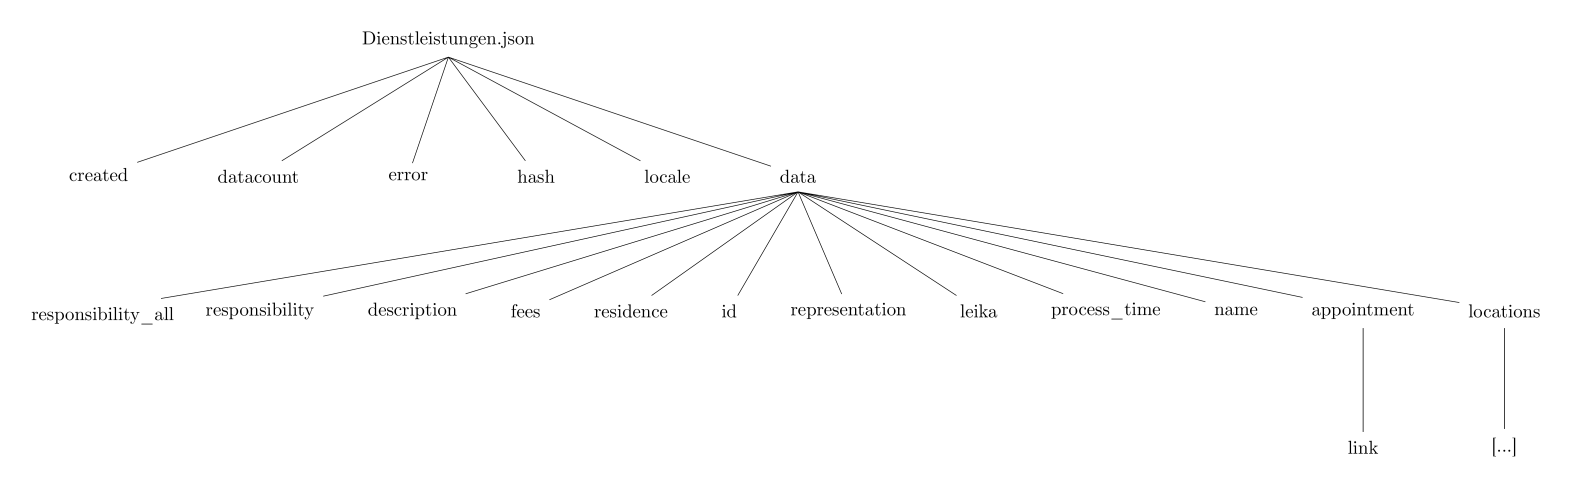
\includegraphics[width=0.9\textwidth]{DLprim}
\end{figure}

\begin{figure}[H]
	\caption[Secondary Nodes of \mintinline{bash}{Dienstleistungen.json} ]{Secondary Nodes of \mintinline{bash}{Dienstleistungen.json} show relevant follow-up nodes to the primary node \mintinline{bash}{locations}}
	\label{LeiKaJSON2}
	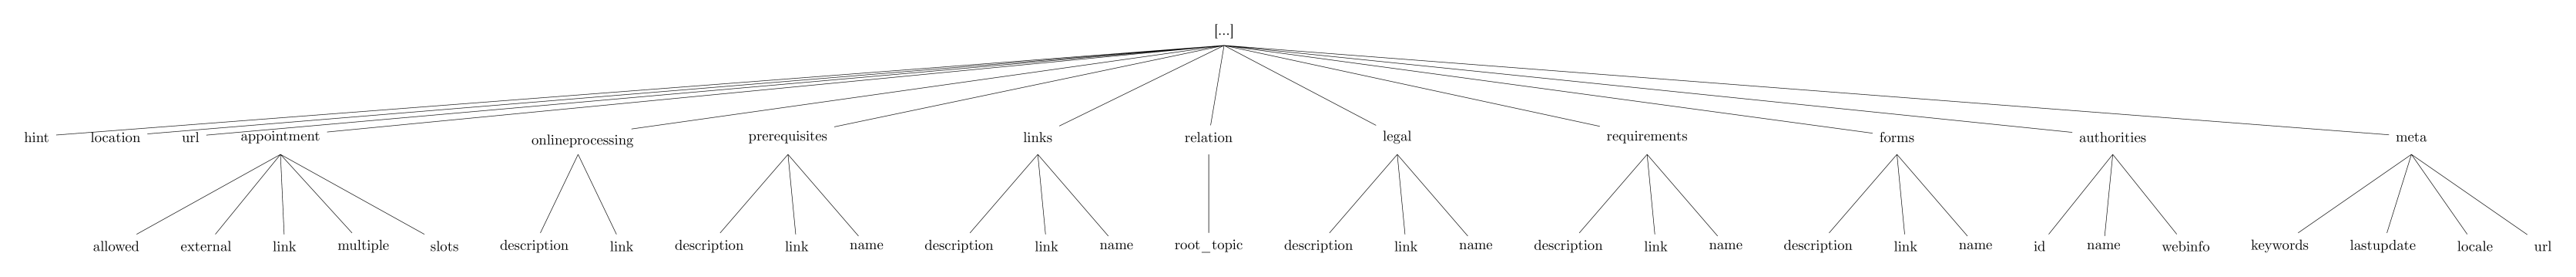
\includegraphics[width=\textwidth]{DLsec}
\end{figure}







\begin{flushleft}


From back-end side, the files mentioned above reporesent cores in a Solr index. The latest version of the underlying Solr server (May 2018) comprises the following cores:

%\begin{itemize}
%	\item 
	\subsection*{\mintinline{bash}{d115}}
%	 :
	 An index core designed to query the latest public services available on Berlin.de. \\ Example services: ``\textit{Personalausweis beantragen} - issuing a passport'', ``\textit{Blindenhilfe} - monetary relief for the blind''.\\  This core initally included 616 nodes at the beginning of this research and now varies between 670 and 680 services depending on the original LeiKa. We will use this core later on as our primary API.
	
%	\item 
\subsection*{\mintinline{bash}{d115Extern}}
%	: 
	An index core designed to include external Hyperlinks outside the service.berlin.de subdomain.\\
	Examples: ``\textit{Gentechnik} - gene technology'' routes to 
	\url{https://www.berlin.de/lageso/gesundheit/gesundheitsschutz/gentechnik/}
	
%	\item 
	\subsection*{\mintinline{bash}{d115Locations}}
%	: 
	An index core designed to query locations of authorities' offices offering a public service and their opening hours\\ %(from the \lstinline|d115| core)
	e.g. ``Kfz-Zulassungsbehörde-Lichtenberg"''
	the authorities' offices and their opening hours.\\
	Based on (\mintinline{bash}{./ssds-data-berlin/json/behoerden/behoerden.json} which will help us indirectly in our implementation later on. 
	
	
%	\item 
	\subsection*{\mintinline{bash}{d115Spelling}}
%	: 
	An index core designed to make the chatbot able to determine spelling mistakes in names of entities (e.g. offices, services) and automatically correct these in the conversation flow
	
%	\item 
	\subsection*{\mintinline{bash}{d115Topics}}
%	: 
	An index core designed to query the database for topics. Each topic collects a set of services that are of the same interest group. For instance, a topic ``Ausländerangelegenheiten'' comprises all sorts of visa and residence permit types. Another topic on ``Auto und Verkehr'' includes services like parking options, paying fines and issuing a driver's licence.
	%trelated .
	
%	\item 
	\subsection*{\mintinline{bash}{smalltalk}}
%	: 
	An index core designed to make the chatbot more interactive by including simple questions and answers to them not related to Berlin.de's service catalogue
	
	
	
%\end{itemize}


\end{flushleft}




Tables \ref{dienstleistung:summary2} and \ref{dienstleistung:summary1} represent the Solr index cores available on \mintinline{bash}{/home/ssds/ssds-solr/data/cores/} and show the fields (child nodes) of each core on Solr, as it is important to have the structure of these files for our implementation.%, the next table contains all %a compact form of each core.
We refer to our Solr instance from now on as the API, since it is built and operates independently from the Groovy web app and only delivers the results to it. Hence, it offers an opportunity to be shared by another programme, rendering it into a standalone API endpoint that can be hosted on its own server as will be discussed in Chapter \ref{maintwo}.

In Table \ref{dienstleistung:descr} we cover an excerpt of most node elements we will later use %more or less in the same structure of the JSON file containing the interaction model:\\
in a similar structure for our own front- and back-end. 

After understanding the links between the API and the sitemap of the Berlin City Portal, we draw a few connections summarised in Table \ref{BerlinSiteMap} to understand how we can proceed with the API and eventually modify or expand it with additional parsers such as Apache Nutch or other runtime parsers (e.g. to find the next appointment, since this is not provided by the API) to suit our voice service solution.







\begin{table}[H]
	\caption[Structure of API]{Structure of API - Solr cores 1-5, version (\textit{ver.}) and relevance (rel.) to our implementation. \textbf{Boldfaced entries} are explained in Table \ref{dienstleistung:descr}}
	\label{dienstleistung:summary2}
	\begin{tabu} to \textwidth{|X[3]|X|X[10]|}
		\hline
		Core Name, \textit{Ver.,} rel. & No. Entries & Fields for each entry (by Order of Child Nodes)\\ \hline \hline
		
	
		
		%can be moved as a cell to next page 0 will then produce one complete page. do not add any extra line lest the page number gets overwritten
		
				\lstinline|d115| \footnotesize{\textit{426,} \quad \quad \quad very relevant} & 672 & 
		\begin{tabu} to 5cm {ll}
			\textbf{\lstinline|id|}  & \textbf{\lstinline|d115Url|} \\ \textbf{\lstinline|d115Name|} &
			\lstinline|ssdsAll| \\ 
			\textbf{\lstinline|d115Description|} & \lstinline|d115Synonym| \\ \lstinline|d115Position| &  \textbf{\lstinline|d115InfoLaw|}\\ \textbf{\lstinline|d115Prerequisites|} &  \textbf{\lstinline|d115Requirements|}\\  
			\lstinline|d115Forms| & \textbf{ \lstinline|d115Fees|}\\ \textbf{\lstinline|d115ProcessTime|} &  \lstinline|d115AppointmentLink| \\ \lstinline|d115ServiceLocations| &  \lstinline|d115ServiceLocationsJson|\\ \lstinline|d115ServiceResponsibility| &  \lstinline|d115ServiceResponsibilityAll| \\  \lstinline|d115OnlineProcessingLink| &  \textbf{\lstinline|leikaId|}\\ \lstinline|leikaName| &  \lstinline|leikaGruppe| \\  \lstinline|leikaKennung| &  \lstinline|leikaVerrichtung| \\ \lstinline|leikaVerrichtungDetail| &  \lstinline|leikaSynonym| \\  \lstinline|ssdsName| &  \lstinline|ssdsLemma| \\ \lstinline|ssdsLongName| & \lstinline|ssdsGruppe| \\ \lstinline|ssdsGruppeDict| &  \lstinline|ssdsKennung| \\  \lstinline|ssdsKennungDict|& \lstinline|ssdsSynonym| \\  \lstinline|ssdsSynonymDict| &  \lstinline|_version_|\\
			
			
		\end{tabu} \\ \hline
		
		
		
		
		
		
		
		
		\lstinline|d115Extern| \footnotesize{\textit{396,} semi-relevant} & 1488 & 
		\begin{tabu} to 5cm {lll}
			\lstinline|id| &  \lstinline|d115Topic| & \lstinline|d115Name| \\  
			\lstinline|d115Link| & \lstinline|d115Keywords| & \lstinline|_version_|\\ 
		\end{tabu}
		\\ \hline
		
		
		\lstinline|d115Spelling| \footnotesize{\textit{678}, semi-relevant}  & 1233 & 
		\begin{tabu} to 5cm {ll}
			\lstinline|id| &  \lstinline|complex object| \footnotesize{(irrelevant)} \\ 
			\lstinline|_root_|  & \lstinline|_version_|\\ 
		\end{tabu}
		\\ \hline
		
		
		\lstinline|d115Topics|  \footnotesize{\textit{426,} semi-relevant} & 167 & 
		\begin{tabu} to 5cm {lll}
			\lstinline|id| &  \lstinline|d115Name|  & \lstinline|d115Path|  \\ 
			\lstinline|d115Keywords| &
			\lstinline|d115Links|  & \lstinline|_version_|\\ 
		\end{tabu}
		\\ \hline
		
		\lstinline|smalltalk|  \footnotesize{\textit{396,} semi-relevant} & 1366 & 
		\begin{tabu} to 5cm {lll}
			\lstinline|id| &  \lstinline|smalltalkAnswers|   &
			\lstinline|smalltalkQuestion| \\
			\lstinline|_root_|  & \lstinline|_version_|\\ 
		\end{tabu}
		\\ \hline
		
		
		
		
	\end{tabu}
\end{table}









\begin{table}[H]
	\caption[Structure of API (cont'd)]{Structure of API (cont'd) - Solr cores no. 6 (last),  version (\textit{ver.}) and relevance (rel.) to our implementation. }
	\label{dienstleistung:summary1}
	\begin{tabu} to \textwidth{|X[3]|X|X[10]|}
		%		& & \\ 
		\hline 
		Core Name, \textit{Ver.,} rel. & No. Entries & Fields for each entry (by Order of Child Nodes)\\ \hline \hline

		
		
		
		
		
		
		
		
		
		
		\lstinline|d115Locations| \footnotesize{\textit{426,} relevant} & 560 & 
		
		\begin{tabu} to 5cm {ll}
			\lstinline|id|  & \lstinline|d115Url|\\ \lstinline|d115Name| &
			\lstinline|d115LongName| \\ 
			\lstinline|d115Type| & \lstinline|d115SuperType| \\ \lstinline|d115District| &  \lstinline|d115SuperDistrict|\\ \lstinline|d115AddressHouseNumber| &  \lstinline|d115AddressCity|\\  
			\lstinline|d115AddressStreet| &  \lstinline|d115AddressPostalCode|\\ \lstinline|d115AddressGeo| &  \lstinline|d115AddressNote| \\ \lstinline|d115AddressUrgentEndDate| &  \lstinline|d115TransitTram|\\ \lstinline|d115AccessibilityElevator| &  \lstinline|d115AccessibilityAccess| \\  \lstinline|d115AccessibilityParking| &  \lstinline|d115AccessibilityWc|\\ \lstinline|d115ContactEmail| &  \lstinline|d115ContactFax| \\  \lstinline|d115ContactPhone| &  \lstinline|d115ContactWebInfo| \\ \lstinline|d115ContactCompetence| &  \lstinline|d115ContactSignedMail| \\  \lstinline|d115ContactSignedMailLink| &  \lstinline|d115Payment| \\ \lstinline|d115PaymentCode| & \lstinline|d115AppointmentNote| \\ \lstinline|d115OpeningTimesMonday| &  \lstinline|d115OpeningTimesTuesday| \\  \lstinline|d115OpeningTimesWednesday|& \lstinline|d115OpeningTimesThursday| \\  \lstinline|d115OpeningTimesFriday| &  \lstinline|d115OpeningTimesSpecial|\\
			\lstinline|d115LocationServices| &  \lstinline|d115LocationServicesJson| \\ \lstinline|_version_|& \\
			
			
		\end{tabu}
		\\ \hline
		
		
	\end{tabu}
\end{table}






\begin{table}[H]
	\caption[URL structure of Berlin.de]{Structure of Berlin City Portal URLs. We use these to collect additional information beyond the API's content (i.e. Solr fields).  \\ Base URL:  \url{https://service.berlin.de/}}
	\label{BerlinSiteMap}
	\begin{tabu} to \textwidth{X[5]|X[3]  X[8]}
%		\hline
		Web Page displays & URL Path & Suffix \\ \hline \hline
		
		a public service & dienstleistung/ & \lstinline|id| \\ \hline
	

		an %municipality / 
		authority homepage & behoerden/ & variable, \quad \space \space no base URL, external link\\	\hline
		
		
			
		a service location & standort/ & \lstinline|d115ServiceLocation|\\ %\hline
		
		
%	\hline	
	\end{tabu}
\end{table}




%htbp
\begin{table}[H]
	\caption[Relevant Nodes in API Query Results]{Relevant nodes in Solr API query results in core \mintinline{bash}{d115}, based on \mintinline{bash}{Dienstleistungen.json} usable in our implementation - at the example of a public service called: ``Fiktionsbescheinigung''}
	\label{dienstleistung:descr}
	
	\begin{tabu} to \textwidth{X[3]|X[11]}
%		\hline
		Key\textless Type \textgreater  & \footnotesize{\textit{ \textcolor{red}{[Omitted Text]}} \textsf{in} \textit{Example Value}}  | Description | \textbf{Remarks on Syntax}  \\ \hline \hline
		
		\shortstack[l]{\textcolor{white}{text}\\\lstinline|id| \\ \lstinline|<int>| }& \shortstack[l]{\textcolor{white}{text}\\ \footnotesize{\textit{326233}} \\ public service ID % on \href{https://service.berlin.de}{service.berlin.de} 
	}\\
		\hline
		
		\shortstack[l]{\textcolor{white}{text}\\\lstinline|d115URL|  \\%URL 
		\lstinline|<string>| } & \shortstack[l]{\textcolor{white}{text}\\ \footnotesize{\textit{https://service.berlin.de/dienstleistung/326233/}}\\
		 link to public service URL % on  \href{https://service.berlin.de}{service.berlin.de} 
		 \\ \textbf{URL structure includes \mintinline{bash}{id} - See Table \ref{BerlinSiteMap} }
	}\\
		
		\hline
		\shortstack[l]{\textcolor{white}{text}\\ \lstinline|d115Name|\\ \lstinline|<string>| }  & \shortstack[l]{\textcolor{white}{text}\\ \footnotesize{\textit{Fiktionsbescheinigung}} % Fiktionsbescheinigung 
		\\ public service name as listed on Berlin.de %\href{https://service.berlin.de}{service.berlin.de/dienstleistungen} 
	}\\		
		\hline
		
%		\shortstack[l]{\textcolor{white}{text}\\ \lstinline|ssdsAll| \\ \lstinline|<string>| } 
%		& \shortstack[l]{\textcolor{white}{text}\\ 
%			\footnotesize{\textit{``Fiktionsbescheinigung'',
%			``Eine [...] ausgestellt, wenn [...] weil \textless br /\textgreater \backslash n \texless br / \textgreater \backslash n \textless ul class= \backslash ``list\backslash ''\textgreater \textless li\textgreater Unterlagen [...]'',}} 
%		\\
%			\footnotesize{\textit{[...], "Visum",	"Fiktionsbescheinigung", "\S 81 \textcolor{red}{[...]} ::: false ::: http://[...]",[...]
%		}
%	}
%		\\ additional captive search terms, synonyms used by \\ Virtueller  Bürgerassistent. Found to be helpful in conversations \\ with the chatbot
%	} \\		
		
		\shortstack[l]{\textcolor{white}{text} \\ \\\lstinline|d115Description| \\ \lstinline|<string>| } & \shortstack[l]{ \textcolor{white}{text} \\
			\footnotesize{\textit{``Eine Fiktionsbescheinigung wird ausgestellt, wenn über einen \textcolor{red}{[...]}''}}\\
			 Introductory paragraph about the service web page \\ 
			\textbf{incl. HTML tags}
	}\\ %like <\backslash br> and <ul ...> \\		
		\hline
%		\inote{uncomment}  \inote{more as} & \inote{needed in next draft}  \\
		
		%		
		%		\mintinline{json}{d115Synonym} & \mintinline{json}{string} & ... & captive search terms, synonyms created by Virtueller Bürgerassistent \\		
		%		
		%		\mintinline{json}{d115Position} & \mintinline{json}{string} & ... & captive search terms, synonyms used by Virtueller Bürgerassistent \\		
		%		
			\shortstack[l]{  \textcolor{white}{text} \\ \lstinline|d115InfoLaw| \\ \lstinline|<string>|} & \shortstack[l]{
					\textcolor{white}{text} \\
					\footnotesize{\textit{\S 81 Aufenthaltsgesetz - AufenthG ::: false ::: http://www.gesetze-im-inter\textcolor{red}{[...]}
					}} \\
					 Legal base for offering this public service
				} \\		
			\hline
		%		
		%		\mintinline{json}{ssdsAll} & \mintinline{json}{string} & ... & captive search terms, synonyms used by Virtueller Bürgerassistent \\		
		%		
		%		\mintinline{json}{ssdsAll} & \mintinline{json}{string} & ... & captive search terms, synonyms used by Virtueller Bürgerassistent \\		
		%		
		%		
		%		
		%		
		%		
		%		
		%		
		%		\mintinline{java}{string} & \mintinline{java}{responsibility}  & denoting in which city halls a service is available\\
		%		\mintinline{java}{boolean} & \mintinline{java}{responsibility_all} & a flag set to true in case the service is available in all local authority offices / service points\\
		%		
		%%	\mintinline{java}{HTML list string} & \mintinline{java}{ description} &  not unified and includes text \\
		%%%		\item  \lstinline|<string> not unified and might need to have an \lstinline|int| added to it and set to 0 in case service is free
		%		\mintinline{java}{int} & \mintinline{java}{residence} & \\
		%		\mintinline{java}{int} & \mintinline{java}{id} & \\
		%		x & \mintinline{java}{representation}  & x\\
		%		\mintinline{java}{long} & \mintinline{java}{leika}  & \\
		%		\mintinline{java}{string} & \mintinline{java}{process_time}  &  need to derive minimum, average and maximum service times instead of a string, as well as conditions\\
		%		\mintinline{java}{string} & \mintinline{java}{name} & the name of the service that would make sense to a human \\
		%		\mintinline{java}{node} & \mintinline{java}{appointment}  &  \\ 		
		%%		% then inner node 
		%%%		\begin{itemize}
		%%%			\item \lstinline|link| (Key value with URL to /terminveinbarung page) - check if orphan or if it is for each beh\"orde and in that case how it gets the right one
		%%%		\end{itemize}	 
		%		\mintinline{java}{node} & \mintinline{java}{locations}  & \\ 
		%%		% then inner node
		%%%
		%%			\mintinline{java}{hint}
		%			\mintinline{java}{int} & \mintinline{java}{sth} & location| one of the 12 authorities \\
		%%%			\item \lstinline|url| of that service at that authority
		%			\mintinline{java}{node} & \mintinline{java}{appointment} & (a second one)	 \\	
		%		\mintinline{java}{node} & \mintinline{java}{onlineprocessing}  & \\
		%		\mintinline{java}{node} & \mintinline{java}{prerequisites} & \\
		%		\mintinline{java}{node} & \mintinline{java}{links} & \\
		%		\mintinline{java}{node} & \mintinline{java}{relation}  & \\
		%		\mintinline{java}{node} & \mintinline{java}{legal}  & \\
		%		\mintinline{java}{node} & \mintinline{java}{requirements}  & \\
		%		\mintinline{java}{node} & \mintinline{java}{forms}  & \\
		%		\mintinline{java}{node} & \mintinline{java}{authorities}  & \\
		%		\mintinline{java}{node} & \mintinline{java}{meta}  & \\
		
		
		
		
			\shortstack[l]{ \textcolor{white}{text}\\\lstinline|d115Prerequisites |%\\%\lstinline|<string>|
			} & \shortstack[l]{
			\textcolor{white}{text} \\
			\footnotesize{\textit{``Persönliche Vorsprache ist erforderlich ::: false ::: '', \textcolor{red}{[...]}
			}} \\
			Conditions a citizen needs to fulfill in order to obtain the service\\
			\textbf{incl. non-fluid text (unique patterns, parsed/encoded HTML)}
		} \\
	\hline
	
				\shortstack[l]{ \textcolor{white}{text}\\\lstinline|d115Requirements |%\\\lstinline|<string>|
				} & \shortstack[l]{
		\textcolor{white}{text} \\
		\footnotesize{\textit{``Bisheriger Aufenthaltstitel ::: Soweit vorhanden, ist der \textcolor{red}{[...]} '', \textcolor{red}{[...]}
		}} \\
		Required document(-s) citizens need to present to obtain service\\
			\textbf{incl. non-fluid text (unique patterns, parsed/encoded HTML)}
	} \\
		\hline
		
						\shortstack[l]{ \textcolor{white}{text}\\\lstinline|d115Fees |\\\lstinline|<string>|
		} & \shortstack[l]{
			\textcolor{white}{text} \\
			\footnotesize{\textit{``Ab dem 01.09.2017:\textless br /\textgreater  \textcolor{red}{ [...]} ''
			}} \\
			Cost of the service\\
			\textbf{incl. non-fluid text (unique patterns, parsed/encoded HTML)}\\
			\textbf{variable free Text for same value, e.g. free services} \\
				\textbf{cannot be explicitly read as primitive data type} \mintinline{text}{int/bool}
		} \\		
		\hline
		
		
		
		
		\shortstack[l]{ \textcolor{white}{text}\\\lstinline|d115ProcessTime |\\\lstinline|<string>|
		} & \shortstack[l]{
			\textcolor{white}{text} \\
			\footnotesize{\textit{``Die Fiktionsbescheinigung wird bei Vorsprache ausgestellt.''
			}} \\
			Time required to process the application for the service\\
			\textbf{incl. non-fluid text (unique patterns, parsed/encoded HTML)}\\
			\textbf{variable free Text for same value, e.g. immediate services} \\
			\textbf{cannot be explicitly read as primitive data type} \mintinline{text}{int/bool}
		} \\		
		\hline
		
		
		
								\shortstack[l]{ \textcolor{white}{text}\\\lstinline|leikaId |\\\lstinline|<int>|
		} & \shortstack[l]{
			\textcolor{white}{text} \\
			\footnotesize{\textit{99010008012000 
			}} \\
			LeiKa identifier as discussed in Section \ref{leikaSec}
%			\\
%			\textbf{incl. non-fluid text (unique patterns, parsed/encoded HTML)}\\
%			\textbf{variable free Text for same value, e.g. free services} \\
%			\textbf{cannot be explicitly read as Integer/Boolean}
		} \\		

		
		
%		\hline
	\end{tabu}
\end{table}
















There are other elements not directly available in the Solr index as fields such as objects from \mintinline{bash}{./ssds-data-berlin/json/districts.json}, which displays each municipality - \textit{Bezirksamt} in relation to the districts - \textit{Ortsteile} and Postal codes - \textit{PLZ} it contains.  As these are helpful to our implementation structure, they make good candidates for a new object type (as discussed later in the interaction model, Chapter \ref{mainone}).  There are some naming ambiguities in the file structure that will need an implicit type inference. For instance, the type of location is only distinct through the name, e.g. `Lichtenberg' for the municipality and `Lichtenberg-sub' for the district.
%related to the districts' locations (PLZ of an Ortsteil, 






\section{The Virtual Citzen Assistant at Runtime}

\begin{wrapfigure}{l}{0.5\textwidth}
	\caption[Simplified Demonstration of Nodes' Traversal]{Simplified demonstration of how nodes are traversed in Virtual Citizen Assistant}
	\label{chatbotnodes}
	\includegraphics[width=7cm]{chatbotnodes}
\end{wrapfigure}



The web app revolves around the following algorithm: once a public service has been caught from the user's input, the chatbot shows the description of the service, followed by a series of questions beginning with a yes/no one to determine if the user is interested in knowing more about the cost of the service, followed by another to pompt if the chatbot should show information of other metadata of the service, e.g. processing time or which authorities are responsible to offering the service. The user navigates by clicking on the links provided inside the chatbot conversation. 
The yes/no questions are translated as \textbf{intents}, which the users either wants to pursue or ignore.

For a yes answer, the chatbot selects child nodes of a node it is currently pointing to, e.g. a service node and checks if it can show their content if these are not empty. If the user chooses not to pursue the intent, the chatbot skips to the next element (or node) in the loaded list from a JSON file as described above. With the modular structure of the nodes, the chatbot is allowed to traverse each service node and metadata nodes to display the proper information as seen in Figure \ref{chatbotnodes}.


The content of these nodes is provided through the %Federal 
IT Service Centre Berlin - \textit{IT Dienstleistungszentrum Berlin, ITDZ} and is part of  %Federal Catalogue of Public Services (
LeiKa%)
. In a similar implementation for the Facebook chatbot Berlina (currently in Beta), Hassmann and Müller \cite{hassmannMlr:berlina} explore a similar implementation and conclude with the use of JSONs being a flexible foundation for development.


% moved leika up^^



%
%\todo{-\textbf{Theorie}\\
%	-summarize LeiKA infobroschuere(BMI08324screenBarrierefrei.pdf)\\
%	-Welche Daten gibt es?\\	  
%	-Was sind die Erwartungen?\\ 	
%}


%\todo{
%	\textbf{current berlin.de bot - What to include?}\\
%	- dienstleistungen.json structure %(finding the info through hierarchical nodes)\\
%	- interpreting the nodes as intents, Solr cores\\
%	- traversing the nodes (one level up then to next node)\\
%	- no session/no persistence\\
%	- explain how the json nodes map to intents and cores in solr etc
	
	%x	x	x
	%ooo ooo ooo
	%try first, go to second (kosten, zeit, rechtsgrundlage, ..) skip one if it has already been suggested.. hinweis..that is built into the xml
	%
	%the live service is different than the one at DAI
	
%	- webapp using groovy\\
%	- what to mention about AllInclusive?
%	- whatever it is, it should go here or before it can go in implementation section.\\
%	- structure of Hitlist on berlin.de  is provided by ITDZ \\
%	- explain LeiKa old and new JSON as an intro to API\\
%}







%\todo {change this into a table and add a tree list like the interaction model in appendix\\




%
%
%\todo{
%	\textbf{API analysis}
%	- missing variables e.g. are required papers, \\
%	- flag: persönliche Vorsprache ja nein, ...\\
%	- started with 616 Intents %in \lstinline|data| node 
%	(now 685 or so), each containing \inote{Tableau}\\
%	- should I include the JSON samples from Appendix here? or just refer to them?}
%














%\todo{\textbf{summary and Ausblick}\\
%	- static system as the Dienstleistungen do not change regularly\\
%	-  as opposed to Versicherungsfirma z.B (ML tries to detect irregular patterns in case customer is lying).\\
%	- 	- no session/no persistence\\
%	- unfortunately forums vs. FAQs did not work. if I want assistance, I want the customer to tell me the model number - and forums have mostly Schrott!\\
%	- what the bot currently achieved is at least not give wrong answers, sometimes says idk but it doesn't confuse you.\\ %same attitude like in lmny shops 
%	- we talked about this in intro chapter. see if you want to mention again with a diff angle\\
%	-(nur unpassende antworten sind frustrierend!)\\
%}

%\subsection*{D115 and The Currently Deployed ``Virtual Bürgerassistent''}
%\todo{
%	- LeiKa

%	-Use case im Detail\\
%	- wie kann man die G\"ute des Systems beurteilen? \textbf{do not forget the survey u made}\\   
%	- Meist sollte man in diesem Kapitel die L\"osung schon im Auge haben, um die Erwartungen so zu formulieren, dass die L\"osung auch geeignet ist?\\ 
%}


\section{Summary}
The Berlin use case is complex in the sense that there are many entangled entities and relationships between the hierarchy of the municipalities. Representing these in one hierarchical diagram is counter-productive due to the rich attributes to numerous special cases and the independence of each authority type of the other. LeiKa overcomes this challenged through a system of sectioned serial number for each office. Yet, understanding how each service operates remains a task to the developer to be able to gather an all-inclusive service strategy for a voice assistant. The modular structure of the Solr API is a helpful tool to send queries and get responses to the software solution we seek. A more in-depth look at the content shows potential adjustments required to adopt it to the solution we present.
We discover that Berlin.de shows features of REST architecture such as unique identifiers for pages representing entities (locations, services) and pagination capabilities throughout the website (e.g. for appointment bookings).

As such, operating a voice assistant as a new service could be delegated to D115 as an authority under the realm of the German Ministry of Interior with the help of the ITDZ, since both entities have the knowledge base and the content to power the service. As the content is subject to changes at any time, updates have to happen without the user having to update in order not to give customers obsolete information. This is part of D115's policy of assuring correct and helpful information is given. For any software solution we present, the guidelines summarized in Section \ref{d115} have to be adhered to. Accordingly, special attention has to be given about data collection. We show in our implementation (Chapter \ref{maintwo}) how we address this by not storing user sessions in any persistent form.
We categorise our system as semi static, since only the content should be interchangeable through an independent API (Solr in our case). 

As per D115's guidelines, we should be able to understand from special cases how to maintain a more well-rounded software that handles more specific cases, and not only give general information. As this requires more detail for requirements engineering (tender and performance specifications), we keep this implement for a future stage. This might involve uses of ML to detect patterns and irregularities

Finally, with human interaction being a favourite option for customers, our software solution competes to present an alternative that is persuasive enough to lure customers to use it. For this, making it constantly available to the user with no waiting time on phone queues or in a public office gives a good starting point. And while the software does not have to understand everything the user says, it should be able to abstain from giving wrong answers at the least in order to yield objectively satisfied customers and no frustrations for receiving misleading or confusing information as discussed in Section \ref{pubsvc}.

%could be held responsible for operating the 





%Modularer aufbau... identical API
%no sessions
%
%see appendix for all code











%###################################################################################
%###################### GUI/VUI ####################################
%###################################################################################

\chapter{The Voice as a User Interface} 
\label{vui}


We start this chapter by juxtaposing the Voice User Interface (VUI) to the Graphical User interface (GUI) respective to cognition and behavioural design which gets us to define new terminological foundation that will follow throughout this thesis.

\section{GUI vs. VUI}
\label{guivsvui}

Visuals and Sounds can both communicate the same message even though they use a  completely different medium. One one hand, the premise that ``a picture is worth a thousand words'' can be valid based on the image but only assumes that we want to give a clear picture to the receiver. Communication through voice, on the other hand, can generally allow more room for interpretation. We think of watching a football game on TV vs. listening to the same game on radio as an example, where listening to it allows each person in the audience group to imagine a different game for themselves, even though the match result are the same.


%%%Image

When we use written text, be it in a document or a street sign, or any label, we seek to mostly assure that all %receivers 
readers understand the same message with a universal codification of what we want to express through the language we use. In this process, language becomes the common denominator for understanding and the short written text becomes purposefully designed to give in the best case a message or instruction not open to interpretation and so a foundation for an agreement or contract between % the 
source and 
%the 
destination of the message. It is a good medium of reference. 

%%%%%%%%%%%%%%%%%%%%%%%%%%%%%%%%%%%%%%%%%%
%voice message in airport - you can do your activity unobstructed
%%%%%%%%%%%%%%%%%%%%%
\section{Utility of Voice}
The utility of Voice comes handy with its different paradigm in numerous settings. 
For a passenger at the airport or an employee between meetings, 
%it is equally as helpful f
%as it would be for a  rushing to a meeting.
it can be more effective to ask questions through conversation than transform them into a query then type them on a screen,
%someone about the information you need quickly if you can ask it in a precise sentence quicker than you would write it, 
or visually navigate on a web page / mobile application until we reach the information we want. In a 2016 Cisco Systems (formerly MindMeld) survey \cite{mindmeldReport}, of 1800 users of voice assistants, 61\% see that the primary use of a voice assistant is when hands or vision is occupied.
Today, this goes further beyond the simple use-cases to become an integral part of our fast-paced life, where we see companies like Ecobee getting around 40 percent of their sales through voice-based AI \cite{mit:Alexa} since their embrace about two years ago. The 10-year-old company's CEO elaborates that their customer “[...] have to fight traffic to get home, and then they have to feed the kids, diaper the baby, and who knows what else. [Ecobee] give them a hands-free way of getting something done while they're in the midst of other tasks” \cite{mit:Alexa} .


Also, in terms of accessibility, blindness could sometimes make voice the only possible way to navigate or be aware of one's surroundings, e.g. a blind person crossing a street depends on the sounds coming from cars and traffic lights.
In that sense, voice can allow people to do their activities free-handed and unobstructed by actively engaging into reading activity %, for instance having to 
as is the case when we look on a screen.
With our ambitions in connectivity becoming more complex, we %have become more 
increasingly started depending on our phones in the last decade.
This is where the use of a Voice User Interface could come at an advantage of liberating us from the constant usage of our smartphones and moving from one screen to another. 
However, it is noteworthy that the trade-off between visually and auditory information exchange comes at a price. While both have their own advantages and disadvantages, it is important to understand that the context in which the medium is used determines dependent factors.

Hence, we need to differentiate between GUI design and that of a VUI. Since most computers and advanced electronic devices operate with a GUI or a simpler textual interface displayed on a screen, our acquaintance with GUI trump the know-how we developed with VUI. %Thanks to the World Wide Web standards with HTML and CSS, 
Therefore, it might not be most intuitive to apply the same concepts on VUI design simply since we start from the mindset that the GUI dictates how to use the software and the user has to understand this interface and deal with it as is.




%\todo{ghaleban mesh mazbouta hena ba3d el refactoring eli 7asal}


%\inote{is this okay here or should it go in an appendix?}
%\sn{andreas doesn't like to have more work done in this part. maybe put some of it in conclusion or remove completely, but i know you won't lol}

\section{Why Can't AI Understand Us}

AI has made giants leaps in the last few years. Thanks to neural networks, Bayesian approaches in classification, decision trees and many other theories, we are capable of performing rigorous analyses on datasets
Considering that speech is one of the most complex forms of data, there are still various challenges that do not have a single strategy to tackle.

\begin{quotation}
What makes voice-based AI so appealing to consumers is its promise to conform to us, to respond to the way we speak—and think—without requiring us to type on a keyboard or screen. That's also what makes it so technically difficult to build. We aren't at all orderly when we talk. Instead, we interrupt ourselves. We let thoughts dangle. We use words, nods, and grunts in odd ways, and we assume that we're making sense even when we aren't. \cite{mit:Alexa}
\end{quotation}

When speech meets AI, there are a lot of language ambiguities to deal with and multiple contexts to understand. Since this is a field by its own and the amount of problems we can face with understanding natural language is unlimited, it is not the scope of this thesis. We only briefly survey a few categorical examples in the following:
\begin{itemize}
	\item \textbf{Sytanx}: homonyms such as ``I \textit{present} you a \textit{present}.'' or ``The \textit{fly} wants to \textit{fly}''
	%homophones, homograph
	
	\item \textbf{Sematics}: metaphors, sarcasm, puns such as ``it's raining cats and dogs''
	
	\item \textbf{Underlying Sentiment}: such as ``oh yeah, sounds very exciting'' when it's not.
	
	\item \textbf{Dialects}: enunciation such as \textipa{[dI"vE|9pm9nt]} \textit{(British)} and \textipa{[d9v"|Apm9nt]} \textit{(Indian)}

\end{itemize}

%\end{itemize}
%
%\begin{table}[h]
%	\begin{tabularx}{\textwidth}{r l l}
%		Syntax & Homonyms & \shortstack[l]{``I \textbf{present} you a \textbf{present}.''\\ ``The \textbf{fly} wants to \textbf{fly}''}\\
%		Semantic & Metaphors
%	\end{tabularx}
%	
%\end{table}
%

%\todo{
%	- \textbf{Why can't robots understand us:} language ambiguities - the need to understand context\\ the Facebook vid\\
%--Syntactical: Homonyme\\ %fly, fly,  presently I'll present you a present - now, give, gift
%--Semantic:  Metaphors, %“it's raining cats and dogs”
%sarcasm, %“oh yea, sounds very exciting”
%and puns\\
%--dialects: enunciations\\
%--underlying grammar\\ %“what makes you abcd just now, ELIZA
%--underlying sentiment\\

%-\textbf{NLP Progress:} How does it help in enriching the bot experience\\
%--neural networks: help understanding language patterns and get better over time\\
%--thought vectors: helps connect different words with related meaingns\\
%--- link: fortschritt, und systemgrenzen heutzutage (kurze Sätze etc)
%}

While Machine Learning enables us to decode phrases not in the classical way in the past by randomly guessing the whole expression, our speech datasets grow and require analysis in further breadth and depth to deliver a sustainable Natural Language Understanding (NLU) engine.
So far, in the past six years our primary approach has changed due to the little progress made with it. Instead of trying to understand exact meanings, we work from
``imperfect matches at the outset, followed by rapid fine-tuning of provisional guesses'' \cite{mit:Alexa}. The learning part is involved by reinterpreting missed expressions \cite{aws:lex_webinar}. 
On one hand, neural networks help us understand language patterns and better the more frequently we use them, but can fail in the case of homonyms. \cite{mit:AILang} Thought vectors, on the other hand, complement them by controlling the connection of different words with their related meanings %, which helps with homonyms for instance.

Mostly independent from the system we use, it is %therefore 
a rule of thumb that most AI-powered personal assistants like Siri or Alexa are %in their 
still at an early learning phase. In order to be able to make use of them in the future, %the %painful 
we need to traverse a period of immaturity teaching the system.
%part has to come in effect. 
This limits us for instance to currently using short sentences to lessen the probability of failure and the system misunderstanding us. And so, naturally, what distinguishes a good system from a better one is how fast it learns.


%a person whos a bit deaf and cant hear us. it happens with ppl too ya3ni}
Interestingly, a side effect of this indeterministic technique is that the voice assistant inadvertently simulates a person who can sometimes not hear us, asks us to repeat a sentence or explain it with different words. Although this is the same idea that a good system should have adequate incoming and outgoing speech fault tolerance, it is unprecedented to tackle a computer system on the consumer level with the idea that we might very much hit or miss the action we want to perform. On the other hand, though premature, it is evidence that a human has much more authority to a machine-powered (and maybe autonomous) brain.


Yet, although it might seem at the beginning that moving between both paradigms is easy, the more detailed system design gets, the trickier it becomes to transform GUI elements into text. Particularly with long texts. We will go over this in more detail about voice design guidelines in Section \ref{designGuide}.



%\todo{ 
%	this is a refactored todo. read in context and see if it fits here\\
%	2 \P \\
	%%%%%%%%%%WILL NOT DO%%%%%%%%%%
%	\textbf{- Chatbot vs. human: }
	%
	%what we used to do with facets vs a search mask predicting possible facets - we are at a stage where bots are like altavista..u tell alexa to open a skill like u tell altavista to look in pics or go to lexisnexis to do reserach. we are yet to reach the state of watson like google is to searches
%	Analyze differences between bot and human response\\
	%human says long sentences and there is a fluid transition between dialog and monologue 
%	-disadvantage: a bot wants a sentence broken down in small pieces to avoid errors in lengthy interpretation\\
	% otherwise, error margin too large.\\
	% this has to do with human language complexity.\\
%}



\section{VUI Semantics}

Having the visual or haptic interface disappear is therefore a game changer for as soon as the user does not have direct instructions on how to deal with it, they start to improvise, or rather move away from the idea that the interface constrains them to the illusion that they define that interface and can control it. For instance, the user knows that they have to press only on a certain area of the screen to activate a button and actively move the mouse to that part. 
%Parallel to this in GUI; 
In other words,
when a user sees a  `save' button on a dialogue box, in their head they relate to it %in their head that 
the functionality of %behind that button lies in 
%of committing 
a commit and keeping a persistent copy of the current state of the parent file to that dialogue. The label `save' describes in a visually expressive fashion what the user can or cannot do within this \textit{dialogue state}.


%Imagine you have an intent resembling the label on th button for ``ok''. with a function linked to it to perform a commit action, ...''}
%  

In voice on the contrary, a user is uninhibited in what they can and cannot say and the system is supposed to understand the \textit{intention} %~\ref{intents} 
of the user with the \textit{formulation} %~\ref{utterances} 
they just used.

%For us to hold on to that sentence, 
In order to translate the aforementioned with less ambiguity, we need to define the lexis we use for voice design utilized in most common chatbot and voice assistants constructs. 
%Just like most common chatbot constructs, Alexa Skills Kit (ASK) 
We divide the building model into \textit{intents}%~\ref{intents}
, \textit{utterances} %~\ref{utterances}
 and \textit{slots} %~\ref{slots}. 
The Fulfilment part is taken care of through a back-end and possibly endpoints connected to it containing the programming and business logic to the interface, which also validate the slots before sending it onwards, similar to when JavaScript takes care of checking a box is not empty when we use a form on% would do on 
a website. %We make the following words clear:

%\sn{Andreas suggests hochstufen - clear split required?}
\section{Terminology}
%Before we discuss our choice of platform in Section \ref{choiceOfPlatform}, 
We already unveiled in Section \ref{approachgoals} that Alexa will be the underlying platform. Thus we cap the elementary definitions of voice assistants with distinct Alexa-specific concepts and give meaning to the following terms: 

	\subsection*{Intent}~\label{intents}
	As the intention the user pursues with a spoken sentence. This translates to the action being executed upon the user's command based on mapping his/her words to this action.
	
	\subsection*{Utterance}~\label{utterances}
	As the wording a user picks to express his intent. For instance, to set the volume on a TV to quieter, we could say ``turn it down a nudge'', ``It's too loud'' or ``lower the volume''. Although all three sentences have the same meaning, linguistically, they are fully unrelated and only context makes us understand them, e.g. we have to know that ``it'' refers to the TV set in close proximity.
	
	\subsection*{Slot}~\label{slots}
	As a variable of a certain type we define in our programme that belongs to a category of items. For instance, when someone says they would like to order a \textit{large} coffee, they assume that there is the option to have a small coffee, too. And so large and small refer both to the size of the coffee. Programmatically, we define \mintinline{java}{large} and \mintinline{java}{small} to be of type \mintinline{java}{size} of the coffee. Similarly, if there is the option to order a tea and a Cappuccino, it would be only fair to define \mintinline{java}{cappuccino} and \mintinline{java}{tea} to be of type \mintinline{java}{beverage}. Consequently, \textbf{slots} can be defined to any part of the sentence, where a parameter (here beverage or size) can be grouped into \textbf{slot types}. 

%\end{itemize}

%avoid using since you won't get indents easily	
%	\begin{minipage}{\linewidth}

	This idea is to be handled with care, though, since technically in most languages we can define a subject, a predicate and an object. Here is an example in English:
	
	% \! for negative spaces in math should be avoided as they do not work consistently
	% check here: https://tex.stackexchange.com/questions/67912/large-negative-spaces
	\[
	\underbrace{I}_\text{subject} \cdot
%	\ \ \ \ \ 
	\underbrace{would \ like  \ to \ have}_\text{predicate} \cdot
	\underbrace{
		\overbracket{a}^\text{number of items} +		
		\overbracket{lar\!ge}^\text{size} +
		\overbracket{cof \mkern-3mu fee.}^\text{beverage}
	}_\text{object} 
	\]
	
	When we design a voice system from scratch, we might have to make it understand how each of these sentence elements can be interchanged with another one of the same slot type. However, since utterances build on they idea of slot types, we can make delegate the system to understand what is important from the sentence through slot types and what other interoperable words are not relevant. In this example, if we say:
	
% \! for negative spaces in math should be avoided as they do not work consistently
	\[
	\overbrace{My \ brother} \cdot
%	\ \ \ \ 
	\overbrace{wants \ to \ order} \cdot
	\overbrace{ a + tall + cof\mkern-3mu fee.}
	\ \ \ \ \ \ \ \ \ \ 
	\]
	
%	\end{minipage}

	it is not important to they system to understand at this stage who is going to drink the coffee. It should be more concerned with the intent; making the coffee, e g. sending a signal or instruction to a coffee machine.
	 
	Ultimately, it is up to us to draw the line on where we want to define a variable slot, that is relevant to the sentence being said by the user in context at a certain time in the conversation flow and where certain sentences would be as a whole giving the same intent
	
	
	\subsection*{Synonym}~\label{synonym:def}
	As a word that has the same meaning of another word that fills a slot. For instance, if we assume that a user says ``I want a \textbf{cup of jolt}'' they system should still be able to understand that they want a standard coffee. If, however, the user defines the type of coffee beans they want, such as `Java' or `Arabica', the system should still be able to differentiate between these and not consider them both as the plain `standard coffee', fulfilling a different intent. 
	
	\subsection*{Dialogue State}~\label{dialogState}
	Like with a state machine, when we have a conversation with Alexa, the dialogue goes into states \mintinline{java}{STARTED}, \mintinline{java}{IN_PROGRESS} or \mintinline{java}{COMPLETED} in the \mintinline{java}{dialogState} property of the JSONs being exchanged with the Alexa client (e.g. an Echo Dot). This is helpful for delegating the dialogue to Alexa or handling it in our own code especially in a %\hyperlink{multiturn:def}{
		multi-turn conversation
%	} 
(see below). More details about this interaction available in the \textsc{ASK documentation} \footnote{\t{a\t{sk}}\href{https://developer.amazon.com/docs/custom-skills/dialog-interface-reference.html\#scenario-delegate}{\lstinline|/dialog-interface-reference.html\#scenario-delegate|}}
	
	
%	\todo{finish these. {More than just Amazon's def}}

	\subsection*{Dialogue Directives}~\label{directives:def}
	Taking advantage of the \mintinline{text}{DialogState} property, dialogue directives are a concept for dialogue management providing a mechanism to conduct dialogues in a multi-turn fashion via Alexa's interaction model directly with little programming effort 
	Without dialog directives, we need to write the logic to collect all the slots (data) we need from users, effectively maintaing the whole session ourselves.
	As such, dialogue directives are a clean way to manage sessions with one of three options: 
	
	\begin{itemize}
		\itemsep0em
		\item Delegating the collecting of required slots to Alexa
		\item handling the multi-turn dialogue in the fulfilment code
		\item using a hybrid of the above.

	\end{itemize}
	
	
	
	\subsection*{Entity Resolution}~\label{entityRes:def}	
	Entity Resolution enables us to use synonyms for slot values without the need to manage this concept in detail in our implementation code. As synonyms are part of the interaction model, resolving them becomes as easy as finding a canonical value in an object (as a complex data type). The concept of entity resolution additionally simplifies verifying that the user indeed said one of the synonyms to a slot value by confirmation utterances from Alexa.\\
	Example: Using entity resolution, we manage to understand \textit{`Perso'} as a synonym to the word \textit{`Personalausweis'} by defining the relationship between both in the interaction model
	
	
	\subsection*{Fulfilment}~\label{fulfillment:def}	
	Building on the intents that the user gives to Alexa, we %need to 
	fulfil the command (after all prompts and confirmations) %. This happens 
	in our back-end code. %Fulfilment is what happens when our back-end code runs. 
	The code itself can vary in implementation using different programming languages %like Java or Python, in 
	or 
	hosting %using our own HTTPS endpoint or a Lambda instance, 
	and the result is what the programme delivers. This is flexible and could range from changing the state of a device, e.g. turning a lamp on to making an API call that delivers text Alexa says. %Programme implementation is very flexible to the developer's needs.
	
	\subsection*{Interaction Model}~\label{interactionMdl:def}
	This is the Skill configuration, also considered as a front-end for the Skill. It is effectively a JSON file of a strict schema that contains all information about what the user says in terms of Utterances, Slots and their types (enumerations of Lists which Alexa tries to resolve our spoken text to). From Alexa's side of speaking, the interaction model only contains the prompts Alexa says to collect slots in the dialog management process (see dialog directives \ref{directives:def})
	
	\subsection*{Multi-Turn Conversation}~\label{multiturn:def}
	A multi-turn (or multi-part) conversation is one, where a dialogue of more than one question and answer takes place. In Alexa's context, this is identified through the \mintinline{text}{dialogState} property and is responsible for collecting / verifying information before it being sent to the back-end for fulfillment.\\
	Example: For the intent \mintinline{text}{transfer_drivers_license}, which includes a required slot that needs the value \mintinline{text}{originOfLicense}, which is of type \mintinline{text}{countryList}, here is a possible 
	
	
	
	\begin{tikzpicture}
	\calloutquote[width=8.6cm,position={(-0.7,0.2)},fill=lightgray!50,rounded corners]{
		
		\textit{``
			Alexa, I want to transfer my driver's license 
			''}
	}
	\end{tikzpicture}
	%\end{quotation}
	%
	%\begin{quotation}
	\begin{flushright}
		\begin{tikzpicture}
		\calloutquote[width=8.9cm,position={(0.5,0.2)},fill=gray!50,rounded corners]{
			\textit{``
				What country is your license issued in?
				''}
		}
		\end{tikzpicture}
	\end{flushright}
	%\end{quotation}
	
	
	%\begin{quotation}
	\begin{tikzpicture}
	\calloutquote[width=3.9cm,position={(-0.7,0.2)},fill=lightgray!50,rounded corners]{
		
		\textit{``
			Mozambique
			''}
	}
	\end{tikzpicture}
	%\end{quotation}
	%
	%\begin{quotation}
	\begin{flushright}
		\begin{tikzpicture}
		\calloutquote[width=7.9cm,position={(0.5,0.2)},fill=gray!50,rounded corners]{
			\textit{``
				Okay, \mintinline{java}{<fulfilment_response>}
				''}
		}
		\end{tikzpicture}
	\end{flushright}
	%\end{quotation}
	
	
	
	
	
		
	\subsection*{Over-answering}~\label{overanswering:def}
	This is what happens when the user provides information that could fill a non-required slot.
	We catch this information by providing all possible utterances a user can say. 
	In the example above, if the  \mintinline{text}{originOfLicense} was not a required slot, Alexa would not prompt us to tell us where the license is issued. If we say in the first utterance to start the intent the name of the country the driver's license is issued in, we over-answer by giving Alexa that information. Depending on our application logic, we can make use of this to make our conversation smarter and not have Alexa ask for information the user already provided, making the voice assistant sound unreliable and primitive. For this, we need to anticipate this effect and include non-required slots in utterances the user might say.

	\subsection*{Persistence and Memory}~\label{memory:def}
	By persistence we mean retention of information that unfolds during a conversation session. As we do not use this concept, we consider our Alexa Skill having no memory, such that it will ask for information it might have asked for before. This is to comply with the D115 guidelines on providing anonymous information and not keeping record or storing any personal data from the user. In general, persistence can happen by storing the session information in a database. For this Amazon recommends the previously discussed DynamoDB (a NoSQL DBMS AWS microservice). Alternatives are open to developers.\\

%%%%%%%%%%%%%%%%%%%%%%%%%%%%%%%%%%%%%%%%%%%%%%%%%%%%%%%%%%%%%%%%%%%%%%%%
%\todo{
%	- how do you think of designing voice when you have a mobile mindset\\
%	- how do you think about screens when you have a mobile mindset and thinking about voice
%	subtle difference
%	
%	- etkallem 3an el paradigm shift eli 7asal ma3 el mouse from cli if not already mentioned\\
%	- then 3an el smartphones and the web from wap etc (deskop version, responsive design, two versions, em instead of pt, relative, starting with a tablet and a phone then anything relative to those then when the standards showed that there won't be an only 15 inch and a 12 inch there will be everything in between, we changed the idea to include continuous units in the spectrum and not only discrete units)
%\cite{alexa_19} \\
%	- different screens, different mobile experiences and what does it mean
%}
%%%%%%%%%%%%%%%%%%%%%%%%%%%%%%%%%%%%%%%%%%%%%%%%%%%%%%%%%%%%%%%%%%%%%%%%

\section{Summary}

In short, 
language is a construct that exceeds the representation of simple expressions in syntax and semantic rules.
Conversation management  %is a very complex 
breaks down the complexity of language and is used in most IVR systems. As we move from building grammars based on Chomskyan theories to resolving parts of a sentence to the nearest elicitations using ML, we introduce concepts and tools to do so. Like in any programming language, concepts need to be defined to have a standardised understanding and not be just related to one language (e.g. type inference is a concept and not a feature in JavaScript).  The interaction model of an Alexa Skill handles a generous amount of implementations to these concepts through a compact tree representation. This helps us to delegate the understanding of user's intents to Alexa as a black box and focus our work more on the fulfilment part. 





%#################################################################################
%###################### State of the Art  ########################################
%%#################################################################################



\chapter{State of the Art}
\label{stateofzart}


This chapter evaluates the possibilities we can combine with the previously discussed artefacts of the Virtual Citizen Asistant. Although we do not exclude a communication with web app at the beginning, we exchange the dependency in favour of the underlying API omitting one layer of communication. We start by positioning our expectations from an AI to then compare the Microsoft Bot Framework, Actions on Google to Alexa Skills Kit as potential underlying systems for our final product.

%\sn{muss evtl weg bzw need to explain relevance}
With these introductory definitions we try to lay out a scaffolding %foundation for a standard, which is still in an experimental phase.
to contain a model for a natural language conversation. Hence we make assumptions on our requirements and explore the options that can suit these. We introduce our requirements in the following Section \ref{choiceOfPlatform} after we understand our current standing point.



\section{Analogies to the Introduction of Web 2.0}

%\todo{web 2.0 was a weird word we didn't use and it became a hype then suddenly it disappeared after it has been defined.\\
%it started with RSS and HTML standards upgrade and now it's totally obvious where it goes.\\
%no one uses RSS, but facebook and the idea of a feed would have not been born have we not started with RSS\\
%}
%
%\todo{	
%	- \textbf{wrap-up:} can bots replace services offered by humans?
%	-- mention transition from facets (AltaVista) to metasearches to all-in-one (Google). \\
%	-- chatbots as enablers in customer service industry\\
%	-- conclusion: Although not impossible, it is a bit too far-fetched at this stage.\\}
%
%\todo{
%	talk about sexism in AI - (why we are still at the beginning)
%}


Much like when tablets and smartphones were introduced to the market, the languages and framework used to render GUIs to the users had to adapt, which resulted into establishing HTML5 and CSS3 as new standards for the web. In that transition, %the experimental phase can be considered when 
browsers had to render different versions of the same page or even different pages depending on the client. It started with a fixed amount of screen resolutions that rapidly grew within a few months. Offering a desktop and a mobile version was another transitory solution paving the way to %and finally to the spreading of 
a display agnostic responsive design. Similarly, the MPEG4 H.264 codec accomplished a better adaptability and less battery consumption for video, which were success criteria to toppling the widespread of Adobe Flash on the web. %and so forth.
When screen sizes and aspect ratios became also so diverse that it was hard to keep track of, websites % designers saw the importance of using different had to be equipped with relative measuring units to present the website correctly (e.g. percentages for CSS classes, ems for fonts, etc.)
adapted in many ways. %To achieve this, many 
The processed can be seen as an organic variation and selection.

With the introduction of VUI for mass consumption and open development, similar undertakings are expected to happen \cite{alexapc18} until we get to acquire an advanced voice user experience. With diverse APIs available explicitly for VUI design, like Bespoken\footnote{\url{https://bespoken.io}} for performance monitoring and testing of a VUI and Sayspring \footnote{\url{https://www.sayspring.com}}
for voice prototyping, we can utilise a few options which are likely to define new modelling and testing standards for VUI design and implementation. At the same time, we expect a few attempts to disappear in the process. Drawing analogies between RSS feeds and the news feed on all social medial platform, we can put the failure of one standard in perspective to the success of another stemming from the same idea. 

As we have seen from previous examples on the web, particularly web searches being the most important, the shift of customers from AltaVista, Lycos, Yahoo! and MSN to Google, Yandex and others shows that marketing, expandability and maintaining quality are key factors to customer retention and survival.



%\todo{should I introduce concepts like entity resolution here already?}











\section[Development Models]{Development Models and Platforms}
\label{devmodels}




\begin{wrapfigure}{l}{0.48\textwidth}
	\caption[VUI-Stack]{The VUI-Stack, showing the different layers a voice service can build on. Based on \cite{voicelabs}}
	\label{vuistack}
	\includegraphics[width=7cm]{Voice-Computing-Market-Map-NextView-1}
\end{wrapfigure}



Chatbots have become available and more accessible to develop through numerous platform (for the same platform (e.g. Facebook), for our own standalone platform(e.g. Lex), or just a tool (Flask)). We no longer have to come up with the whole infrastructure.




This gets us to understand that while it is possible to build a voice service from the ground up, all major platforms already supply the necessities to develop for an existing platform such that a lot of overhead is already implemented. VoiceLabs defines this as the VUI Stack (Figure \ref{vuistack}).

Further, with each of the voice assistants platform becoming specialised in a different domain, %in a certain abilities
it s not suprising to see synergy effects on the market. Recent news about
%	-this could belong here or somewhere else\\
Amazon and Microsoft agreeing to make their voice assistants talk to each other \cite{amznMicrosoft} is one such comparison to how different operating systems today exchange common file formats to do the same tasks differently\\


\subsection*{From End-Users' Point (Convenience and Purpose)}

Before we evaluate platforms in terms of software development, we research the question of evaluating the platform from the customer's point of view. For this we look into empirical data from previous evaluations, then complement it with our own survey. 

In his thesis project, Osman \cite{osman:siri} surveys Siri, Cortana and Google Assistants with respect to their user-friendliness using Attrakdiff and other procedures. The research quantifies perceptions of 24 interviewees (13 women and 11 men between 18-35 years of age) about the voice,  the human aspect of the voice assistant, pragmatic, hedonistic and other qualities. It also tests the reactance of the subjects with ratios about knowing vs. using the voice assistant.

Though the research does not recommend a certain platform, it hints that different platform adapt a different characteristic (especially with regard to wit practicality), which trigger different emotions on different users. Already in 2016, the study shows that the names of the three voice assistants sound familiar to the sampled subjects.

Given its reputation among assistants, Siri has been criticised for its inflexibility and often not understanding more specific commands. Dormhel suggests improvements on translations from English \cite{dormhell:siri} which discourages us to develop for the platform in German if it has a weak foundation.

Other sources indicate that ``AI platforms by Google, Apple, Microsoft, and Amazon all show different strengths. Google Assistant is the best on wide-ranging search commands.'' \cite{mit:Alexa} %Apple’s Siri and Microsoft’s Cortana have other talents. 
As Alexa is particularly talented with shopping commands \cite{mit:Alexa}, the platform revolves well around sustaining a conversation''. %does particularly well with shopping commands.

Quoting Microsoft product manager about Alexa, we acknowledge that ``Alexa’s broader success resides in its ability to alleviate the stresses of an overbooked life. It’s the companion that’s always ready to engage''\cite{darrenAustin}.

Additionally, there are a few plugins in the making to create a voice profile for Google and Alexa, giving an individual touch of sound based on a profile \cite{alexa_19}. This can have a wide-reaching  audience, for instance a voice assistant could mimic the sound and language of a person when they are not present. Likewise, a game can have a richer experience with its characters having different sounds.

%
%\todo{
%	
%	from a user point of view:\\
%	\url{https://www.technologyreview.com/s/608571/alexa-understand-me/}
%	SUSTAINED CONVERSATION\\
%	In studies, \\
%	
%	
%}

\subsection*{From Developer's Point (Cost and Availability)}

The perspective of third-party development focuses mainly on availability of APIs and SDKs. With the exception of Siri being tied to a relatively closed platform and require knowledge of Swift or ObjectiveC, Siri can only be executed if an app is installed on the iOS device.
%an SDK for developing apps that are installed on the iOS devices and 
Moreover, a 99 US\$ one-time fee to become an active developer able to publish on the AppStore is a prerequisite.
Likewise, Microsoft's Azure Services are available with a 30-day trial period, followed by a subscription scheme.
Alexa and Google demonstrate more flexible models with a free tier option %the option to not need to pay any fee 
until after the 3rd-party software is in production. This is another reason that gets us attracted to both platforms. Further, with Alexa and AWS, promoting ads that play from within the Skill has additional costs, but there is a possibility for developers to make a small profit from the Skill once it gets a substantial user base. A developer's guide is available in English and partly in German.

Also, their larger user base promise a higher likelihood for a developed solution to be used on the respective hardware (Android devices, Alexa-enabled devices).
Especially with Amazon Skills launching in Germany only since February 2017, we expect that our solution could fill a market gap. Figure \ref{skillsbyvol} demonstrates how an Alexa Skill could cater for an unsaturated market.




\begin{figure}[h]
	\caption[Alexa Skills by Volume (2016)]{Alexa Skills by Volume (2016) \cite{voicelabs:trends}. Categorised as part of the `local' section, the percentages demonstrate how an Alexa Skill as a choice could cater for an unsaturated market.}
	\label{skillsbyvol}
	\includegraphics[width=\textwidth]{AlexaPie1} 
\end{figure}


As the motivation behind this project is partly to evaluate development for an e-Government service on a new platform, with the Google assistant the option of using Dialogflow\footnote{\url{https://dialogflow.com/}} (formerly API.ai) was excluded as it was explored in the equivalent project by Hassmann and Müller \cite{hassmannMlr:berlina}.\\



With Amazon having an obscure position to data and privacy as opposed to Apple and Siri, this gets us to question how Amazon protects personal data. During the first AWS Public Sector Summit 2018 in Brussels, Belgium with a considerable presence of the European Commission in panels, presentations and workshops, many answers were provided clearing doubts about the company's compliance to the GDPR and its Cloud Computing Compliance Controls Catalog (C5) attestations as a proof % of high standards 
for different forms of data protection (e.g. resale to
 %partners and 
 third-parties and responsibility on cyberattacks) \cite{aws:pubsecsum}
\subsection*{Conducted Survey}

%In addition, 
We survey 34 persons to validate our choice out of the preliminary interest in Alexa. 


The survey aims at understanding potential customers' expectations while evaluating their current understanding of the possibility of a voice assistant for the e-Government sector. Titled `Usability of Voice Assistants', it is divided into the following question sets related to:

%
%\begin{table*}[H]
%	\begin{tabu} to \textwidth {X X}





\begin{table}[H]
	\begin{tabular} {l l}
		
%				&
%		\shortstack{question about if the \\ Virtual Citizen Assistant was used} \\
		
- Demographics &
-	Use of a Voice Assistant  \quad\quad    - Alexa Skills \\	  
-	Berlin.de City Portal &
- 	Alexa as a Voice Assistant \\
-	Voice Assistant for public services  &

-	Linguistic Nuances (Utterances)\\
%	&
%		\includegraphics[width=5cm]{questi/q3}\\
	\end{tabular}
\end{table}
%
%
%
%\begin{wrapfigure}{r}{0.4\textwidth}
%	\caption[Survey Results]{Survey results}
%	\label{sur1}
%	\includegraphics[width=7cm]{questi/q3}
%\end{wrapfigure}
%
%
%\begin{wrapfigure}
%	\centering
%	\caption[Voice Trends]{Trends of increasing use of voice as 
%		\includegraphics[height=5cm]{} 	
%		
%	\end{figure}


%
%\begin{flushleft}
%
%\end{flushleft} 
%&

%	\end{tabu}
%\end{table*}



%
%


%\begin{figure}[b]
%	%	\centering
%	\caption[Survey Results]{\textsc{Demographics \& Use of a Voice assistant} - Results of conducted survey for 34 participants for the development of an Alexa Skill}	
%	
%\end{figure}



\begin{figure}[h!]
	\centering

\caption[Survey Results - Demographics \& Use]{\textsc{Demographics \& Use of a Voice assistant} - Results of conducted survey for 34 participants for the development of an Alexa Skill}




	\begin{subfigure}[b]{\linewidth}
	%		\caption[Global Monthly Active Users (Social Media vs. Messaging Apps]{Global Monthly Active Users \\ in Millions \cite{businsider}}
	\includegraphics[width=\linewidth]{questi/0}
\end{subfigure}



	
	\begin{subfigure}[b]{\linewidth}
		%		\caption[Global Monthly Active Users (Social Media vs. Messaging Apps]{Global Monthly Active Users \\ in Millions \cite{businsider}}
		\includegraphics[width=\linewidth]{questi/1}
	\end{subfigure}
	
	
	
	
		
	\begin{subfigure}[b]{\linewidth}
		%		\caption[Global Monthly Active Users (Social Media vs. Messaging Apps]{Global Monthly Active Users \\ in Millions \cite{businsider}}
		\includegraphics[width=\linewidth]{questi/2-0}
	\end{subfigure}
	

	\begin{subfigure}[b]{\linewidth}
	%		\caption[Global Monthly Active Users (Social Media vs. Messaging Apps]{Global Monthly Active Users \\ in Millions \cite{businsider}}
	\includegraphics[width=\linewidth]{questi/2-1}
\end{subfigure}	
	
	
	
	

\end{figure}




\begin{figure}[p]
	%	\centering
	\caption[Survey Results - Berlin City Portal and Chatbot]{ \textsc{Berlin.de City Portal, the Virtual Citizen Assistant and Activities on Alexa} - Results of conducted survey for 34 participants for the development of an Alexa Skill}
	

			

	
	
	

%\begin{subfigure}[b]{\linewidth}
%	%		\caption[Global Monthly Active Users (Social Media vs. Messaging Apps]{Global Monthly Active Users \\ in Millions \cite{businsider}}
%	\includegraphics[width=\linewidth]{questi/}
%\end{subfigure}	
%
%




\begin{subfigure}[b]{0.3\textwidth}
	%		\caption{Voice-First \\ Device Footprint \cite{voicelabs}}
	\includegraphics[height=6cm]{questi/q1} 	
\end{subfigure}
\begin{subfigure}[b]{0.3\textwidth}
	%		\caption[Global Monthly Active Users (Social Media vs. Messaging Apps]{Global Monthly Active Users \\ in Millions \cite{businsider}}
	\includegraphics[height=6cm]{questi/q2}
\end{subfigure}
\begin{subfigure}[t]{0.39\textwidth}
	%		\caption[Global Monthly Active Users (Social Media vs. Messaging Apps]{Global Monthly Active Users \\ in Millions \cite{businsider}}
	\includegraphics[height=3.8cm]{questi/q3}
\end{subfigure}





	
\begin{subfigure}[b]{\linewidth}
	%		\caption[Global Monthly Active Users (Social Media vs. Messaging Apps]{Global Monthly Active Users \\ in Millions \cite{businsider}}
	\includegraphics[width=\linewidth]{questi/4}
\end{subfigure}




\begin{subfigure}[b]{\linewidth}
	%		\caption[Global Monthly Active Users (Social Media vs. Messaging Apps]{Global Monthly Active Users \\ in Millions \cite{businsider}}
	\includegraphics[width=\linewidth]{questi/5-1}
\end{subfigure}


\begin{subfigure}[b]{\linewidth}
	%		\caption[Global Monthly Active Users (Social Media vs. Messaging Apps]{Global Monthly Active Users \\ in Millions \cite{businsider}}
	\includegraphics[width=\linewidth]{questi/5}
\end{subfigure}


\end{figure}







\begin{figure}[h!]
\begin{center}
	\caption[Survey Results - Activities on Alexa / Assistant for Berlin]{ \textsc{Activities on Alexa and a Voice Assistant for the city's authorities} - Results of conducted survey for 34 participants for the development of an Alexa Skill}




\begin{subfigure}[b]{\linewidth}
	%		\caption[Global Monthly Active Users (Social Media vs. Messaging Apps]{Global Monthly Active Users \\ in Millions \cite{businsider}}
	\includegraphics[width=\linewidth]{questi/6}
\end{subfigure}





\begin{subfigure}[b]{\linewidth}
	%		\caption[Global Monthly Active Users (Social Media vs. Messaging Apps]{Global Monthly Active Users \\ in Millions \cite{businsider}}
	\includegraphics[width=\linewidth]{questi/6-2}
\end{subfigure}


\begin{subfigure}[b]{\linewidth}
	%		\caption[Global Monthly Active Users (Social Media vs. Messaging Apps]{Global Monthly Active Users \\ in Millions \cite{businsider}}
	\includegraphics[width=\linewidth]{questi/7}
\end{subfigure}


%
%
%\begin{subfigure}[b]{\linewidth}
%	%		\caption[Global Monthly Active Users (Social Media vs. Messaging Apps]{Global Monthly Active Users \\ in Millions \cite{businsider}}
%	\includegraphics[width=\linewidth]{questi/7}
%\end{subfigure}



\begin{subfigure}[b]{0.7\linewidth}
	%		\caption[Global Monthly Active Users (Social Media vs. Messaging Apps]{Global Monthly Active Users \\ in Millions \cite{businsider}}
	\includegraphics[width=\linewidth]{questi/8}
\end{subfigure}
%
%
\begin{subfigure}[b]{0.29\linewidth}
	%		\caption[Global Monthly Active Users (Social Media vs. Messaging Apps]{Global Monthly Active Users \\ in Millions \cite{businsider}}
	\includegraphics[width=\linewidth]{questi/9}
\end{subfigure}


%
%\begin{subfigure}[b]{\linewidth}
%	%		\caption[Global Monthly Active Users (Social Media vs. Messaging Apps]{Global Monthly Active Users \\ in Millions \cite{businsider}}
%	\includegraphics[width=\linewidth]{questi/9}
%\end{subfigure}
%
%
%
%
\begin{subfigure}[b]{0.3\linewidth}
	%		\caption[Global Monthly Active Users (Social Media vs. Messaging Apps]{Global Monthly Active Users \\ in Millions \cite{businsider}}
	\includegraphics[width=\linewidth]{questi/12}
\end{subfigure}
%
%
\begin{subfigure}[b]{0.3\linewidth}
	%		\caption[Global Monthly Active Users (Social Media vs. Messaging Apps]{Global Monthly Active Users \\ in Millions \cite{businsider}}
	\includegraphics[width=\linewidth]{questi/10}
\end{subfigure}
%
%
%
\begin{subfigure}[b]{0.29\linewidth}
	%		\caption[Global Monthly Active Users (Social Media vs. Messaging Apps]{Global Monthly Active Users \\ in Millions \cite{businsider}}
	\includegraphics[width=\linewidth]{questi/11}
\end{subfigure}
\end{center}


\end{figure}



\clearpage

The survey is carried out using LimeSurvey, an open tool (for educational purposes) with extensive analysis tools and the ability to export to statistics software such as R, SPSS and any tool accepting CSV file format. It lays out a foundation for future metrics if used in parts and on larger amounts of interviewees.

By combining responses from two or more questions, we find correlations that give us the following key findings: 

\begin{itemize}
	
	\item There is an equal demand for German and English as the VUI language.
	
	\item There is an existing user base for the Virtual Citizen Assistant that has potential to grow and extend to a voice assistant.
\end{itemize}
%
%Further, the utterances section help us diversify the output of the voice assistant.\\


We therefore decide to build an Alexa Skill after having confirmed that the number of users who have heard of Alexa and are using a VUI are the highest.


% into the platform choice, 


%
%\todo{\textbf{by platform:}\\
%	-API.ai \\
%	Facebook Messenger Chatbots \\
%	-wit.ai \\
%	-motion.ai / Flask\\
%}


%\todo{moved from intro (was too detailed for up there):\\
%	- like Siri, Bixby, etc. \inote{put bixby somewhere else and be more precise on what u did based on section choice of platform} \\
%	- such as Microsoft Azure Bot Framework, Amazon Lex and API.ai,
%
%	- some screenshots from Azure etc.\\
%	
%}
%
%\todo{Seif's BA!}






%
%
%
%\todo{
%	Deep Learning (cp)\\
%	
%	There’s an obvious problem with applying deep learning to language. It’s that words are arbitrary symbols, and as such they are fundamentally different from imagery.
%	https://www.technologyreview.com/s/602094/ais-language-problem/
%	. Two words can be similar in meaning while containing completely different letters, for instance; and the same word can mean various things in different contexts.
%}

%%%%%%%%%%%%%%%%%%%%%%%%%%%%%%%%%%%%%%%%%%%%%
\section{Choice of Platform} %comparison AWS vs. el ba2i
\label{choiceOfPlatform}

After deciding that the voice assistant solution will take the shape of an Alexa Skill, we cover here some structural conditions we anticipate with this decision.

%\begin{itemize}
%	\item[
	\subsection*{Secure Data Transfer}
%	] 
	Using Alexa Skills require a secure HTTPS endpoint. As AWS Lambda is a possible option (as a trusted trigger), we consider it in order not to have to manage any SSL certificates (except for at our API). For Lambda, the first million calls a month are for free. Charges apply per 10ms unit.
	
	
%	\item[
	\subsection*{Microservices as Building Blocks} %and Helpers}
%	] 
	While we can use our own building blocks, AWS offers a good combination with the Alexa Skills Kit, from asset hosting to availing virtual machine instances. 
	

%	\item[
	\subsection*{Availability based on Language and Local Store}
%	] 
based on an excerpt from ASK documentation: Availability \footnote{\t{a\t{sk}}\href{https://developer.amazon.com/docs/custom-skills/develop-skills-in-multiple-languages.html}{\lstinline|/develop-skills-in-multiple-languages.html|}} of a Skill depends on the Amazon store selected. An Amazon store is linked to the primary shipping address on the account if provided, otherwise it depends on the initial settings provided through the device from which an account was set up from (e.g. IP-Address, device language settings). With our configuration set to German, 
%	
%	\begin{itemize}
%		
%		\item \space 
[A Skill hosted on the German store only with an interaction model in locales `de\_DE' and `en\_US' can be made] \space available  [.. with the] selected country distribution [before deployment] \cite{alexaDesignGuide}.
It can be used with an account linked to the German store to a device language set in German (Germany) or English (U.S.) 
%		\item \space[It] can be used by customers in Germany who have set their devices to use German.
%		\item \space[It] can be used by customers in Germany who have set their devices to use English (UK).
%		\item \space
		[It] cannot be used by customers in Germany who have set their devices to use English (U.K.) or any other language
		%.
%		\item \space [It] cannot be used by customers 
		and not by an account with German (Germany) or English (U.K.)
		in any other country, regardless of the language they've selected for their devices.
		
%	\end{itemize}
	
	
	
	%	\item[
	\subsection*{Programming Language}
	%	] 
	Choosing a programming language is relevant %, as we have an 
	with respect to the already implemented template of %the 
	Virtual Citizen Assistant %which we want to use 
	intended to extend. At the same time, trying out a new language is a key incentive to start this project. Given that we have the %freedom of 
	choice with Alexa Skills between Java, Node.js framework (JavaScript), C\# and Python, we look at available resources for each language. Node.js proves to be the most resourceful as will be discussed in Chapter \ref{maintwo}. As a secure alternative, the Alexa SDK for Java comes second to Node.js's as opposed to C\#, for which no Alexa SDK exists. With Java and ECMAScript having similar syntax, the arguments to develop on this framework is strengthened.
	
%\end{itemize}



%we wanted something that is close enough to java in case we can use the methods in there but not java 3ashan neghayyar
%
%	- bec. AWS is a whole established ecosystem.
%

% , i.e. objects  had to be redefined since these 
%we made the decision based on Seif' bachelorarbeit

%we want to use as much code from Virtual Citizen assistant as possible

%\todo{I'll have to introduce Skills `officially' in this section for the first time (mentioned already with Georgia as app-like).\\
%	reference it in glossary in two places. here and later in Alexa + skills
%}

%
%\todo{
%	here you can talk about alternatives like Microsoft, etc, compare \textbf{pricing scheme}, say why you chose Alexa (for its popularity mainly and because Api.ai was used in prev. proj.\\
%	%-AWS Lambda is free for the first one million calls per month\\

%	- \url{https://developer.amazon.com/blogs/post/Tx213D2XQIYH864/announcing-the-alexa-skills-kit-for-node-js} having an SDK is very imp (unavailable for C\# e.g.)\\


	
%	- on top of that, alexa does this cool thing where it gives\\
	
%}


%
%
%Before deciding to develop for Alexa, we consider several options and evaluate their advantages and suitability for our requirements.
%
%\todo{elaborate on pricing model in details}
%
%\begin{table}[H]
%	\begin{tabularx}{\textwidth}{r | l l l}
%		& Alexa  & API.ai & Microsoft Azure \\ \hline
%		price & free \footnote{Creating the skill is free, if using AWS to host the backend part (via Lambda): First million calls free per month} & free & free \\
%	\end{tabularx}
%\end{table}
%


%%%%%%%%%%%%




%%%%%%%




%
%
%With Alexa as our choice, we agree to acknowledge the following considerations:
%
%




%%%%%%%%%%%%%%%%%%%%%%%%%%%%%%%%%%%%%%%%%%%%%












%%%%%%%%%%%%%%%%%%%% choice of platform is kinda lost to where it belongs
%%%%%so we move it here for now to make a small intervention between terminology before we move on to alexa in detail
%%%%%%%%%%%%%%%


\section{Summary}

We understand the choice of platform is significant at an initial stage, since it decides on the architecture of the software we develop with. Given that we will have a constraint related to the number of users, we find through the conducted survey that Alexa Skills Kit and AWS are worth embracing as a bilateral ecosystem, to users and developers. Presenting the tangible options that have an interesting relationship with our use-case due to the spread of the platform or our predictions in its relevance as discussed through the comparative literature and preliminary survey results,
in the next chapter, we familiarise ourselves with potential and limitations of this choice.
We also have a questionnaire available for deeper analysis using the statistical indices obtained. With Likert scales modi and mean, the involved correlations can give us further predictions about potential use.





%%%%%%%%%%%%% %%%%%%%%%%%%% %%%%%%%%%%%%% %%%%%%%%%%%%% %%%%%%%%%%%%% %%%%%%%%%%%%% 








\chapter{Amazon's Ecosystem}
\label{amznecosys}

%
%\todo{%remove much from last section above \\
%	 After having a sneek peak into Alexa Skills,we proceed by comprehending the backbone that operates it ...}


% alexa from user and developer sicht

After having a sneek peak into Alexa Skills,we proceed by comprehending the backbone that operates it.
In this chapter we discuss Amazon's state-of-the-art strategy
%before moving on to related work in other archetypes 
as it is important to introduce the implementation scope of voice assistants 
top down
%bottom-up 
prior to exploring the current context 
%within the same boundaries of voice assistants 
%then 
after comparing it to other approaches in the larger context of conversational bots as a whole from a technical and user experience point of view. 


\section[Amazon Web Services + Alexa]{Amazon Web Services (AWS) + Alexa}


Getting started with Alexa as a platform for the first time might seem a little overwhelming especially since each component of it is being  constantly restructured since its debut release in November 2014 and with Q4 2016 being the beginning of its major market penetration success \cite{gartnerpreds17}. % AWS is constantly working on the interface and the sdk 
As throughout the course of this thesis these major changes occurred, we discover that Amazon's philosophy and success is based on the divide and conquer principle on  a large scale. This allows loose coupling of all sorts of components of the company, starting from their business logic to even their branding themes. %including even logo changes of the AWS modules!
%do some kind of changelog later
 

\subsection*{AWS}
Amazon Web Services is a Cloud Computing service provider with a complete set of services to help build and run web applications ``reliably and securely at a cost and scale'' according to one's independent needs \cite{aws_website}.
It comes with agile abilities to adjust to various solution at a flexible scheme with benefits like multiple server farms globally (operating under different legal contracts with respect to data security and user privacy), caching, NoSQL, DevOps and so forth.


\subsection*{Alexa + Skills}
\label{alexa:def}
Alexa is a cloud-based voice service assistant platform by Amazon powering millions of devices %\inote{with \{number of requests\} {daily|monthly}} 
on its own-branded IoT devices like the Echo, Echo Dot, Tap, FireTV as well as cross-platform through mobile apps available through  \href{https://itunes.apple.com/de/app/amazon-alexa/id944011620?l=en&mt=8}{Apple's AppStore for iOS} and  \href{https://play.google.com/store/apps/details?id=com.amazon.dee.app&hl=en}{Google Play Store for Android} devices. Unlike Apple's approach with Siri for instance \footnote{as know from its policy on  new software and hardware products like the case with the iPhone, the Mac and its other product lines}, where including support for third-party integration on iOS's Service Development Kit (SDK), Amazon decided with the launch of Alexa to include non-Amazon developers right from the start by introducing a multitude of (SDKs) around the platform as part of AWS, e.g. Alexa Skills Kit SDK discussed further below.

So far, though the separation of AWS and Alexa's environments is not linguistically intuitive with the company's name labelled on every service component \footnote{see Etymology in Annex \ref{etymology}}, \href{http://www.amazon.com}{Amazon.com, Inc.} offers an array of web services through AWS that summarize all building blocks necessary to operate Alexa as a software for end-users. Of course with the introduction of the aforementioned devices, it becomes intuitive to call these `Alexa devices' since their primary purpose is to operate as Alexa clients. We refer to Alexa here only as the service offered by Amazon to consumers. Consequently, although Alexa comes as a fully packaged service to end-users, we can reduce it to a compilation of many micro-services provided by AWS. As most of these are available separately in the form of Software as a Service (Saas), we conclude that AWS incorporates the following components required to make Alexa come together and becomes a consumer of its own web services platform. 





%\cleardoublepage

\section{AWS Modules as Alexa's Building Blocks }
\label{aws:modules}
%\todo{Legend: Module logos in Illustrator - they are used in graphic beneath}
%\inote{make logos as minipage objects or set as table / problem with footnotes}
%\inote{in print, make sure the following list goes on a spread (odd then even page number) with the image at the end of it for clarity}

listed in sequential order of importance, Alexa's service modules include but are not limited to: 

%\begin{enumerate}



%	
%	\begin{restoretext}
%		\begin{flushright}
\begin{wrapfigure}[2]{r}{1.2cm}
	
\includegraphics[width=1.1cm]{awslogos/lexlogo}
\end{wrapfigure}
%		\end{flushright}
%
%	\end{restoretext}


%	\item[
\subsection*{
	\href{https://aws.amazon.com/lex/}{\textbf{Lex}} \footnote{\url{https://aws.amazon.com/lex}}
%	] 
}
	\textit{for conversational interfaces using Natural Language Understanding, Text-to-Speech and Speech-to-Text} \\
	``a service for building conversational interfaces into any application using voice and text''\cite{aws_website}.
	Lex is the most important backbone to make Alexa possible and can be a main operator of another software package to create a whole new category of independent voice assistants and conversational bots. Independence denotes that  from a VUI Stack like Alexa's with the Echo devices and respective platform, software (Skills and APIs) built on top of it, or with  Siri, where the Hardware is the iOS-operating device and the software being an extension of the mobile apps using Apple's SDK. It would also mean adopting the Alexa API to a new kind of hardware, such as cars, which goes beyond the scope of this work. And while this independence means more flexibility in developing a solution of our own, this would often mean a much higher effort since we miss the opportunity of taking advantage of the already built and tested artefacts. The most critical argument against development with Lex directly is that it was not available in German at the time of this research. We therefore decide to use the Alexa Skills Kit with Alexa as a product and not as API, which ultimately takes advantage of Lex and the other components described below under the hood while still remaining in a familiar and commonly used environment. Lex and Alexa use the same deep learning techniques for natural language processing with the workflow described with the example in Figure \ref{lex_interactionExample} below. Lex's difference to Alexa  is discussed in Appendix \ref{lexAlexa}.


%	
%	\begin{restoretext}
%		\begin{flushright}
\begin{wrapfigure}[2]{r}{1.2cm}
		
\includegraphics[width=1.06cm,height=0.9cm]{awslogos/pollylogo}
\end{wrapfigure}

%		\end{flushright}
%	\end{restoretext}


%	\item[
\subsection*{
\href{https://aws.amazon.com/polly/}{\textbf{Polly}} \footnote{\url{https://aws.amazon.com/polly}}
%] 
}
\textit{for speech synthesis\\}
	another ``service turn[ing] text into lifelike speech, allowing [developers] to create applications that talk'' \cite{aws_website} wile harnessing the power of deep learning. It is more or less the mouthpiece of Alexa built on top of speech synthesis algorithms.
	

	
	%	
	%	\begin{restoretext}
	%\begin{flushright}
	\begin{wrapfigure}[2]{r}{1.2cm}
		
\includegraphics[width=1.4cm]{awslogos/transcribelogo}
	\end{wrapfigure}
	
	%\end{flushright}
	%	\end{restoretext}
	
	%	\item[
	\subsection*{
		\href{https://aws.amazon.com/transcribe/}{\textbf{Transcribe}} \footnote{\url{https://aws.amazon.com/transcribe}}
%		]
} 
		\textit{for automatic speech recognition using Speech-to-Text}\\
	which ``makes it easy for developers to add speech-to-text capability to [...] applications'' \cite{aws_website}. With Transcribe we are able to get text out of the user's voice before passing it into a format Alexa's backend would understand.
	
	
	
	%	
	%	\begin{restoretext}
	%\begin{flushright}
	\begin{wrapfigure}[2]{r}{1.2cm}
		
\includegraphics[width=0.8cm,height=0.9cm]{awslogos/lambdalogo}
	\end{wrapfigure}
	
	%\end{flushright}
	%	\end{restoretext}
	%
	
% \todo{don't mention I'm using lambda until design chapter 3}

%	\item[
\subsection*{
	\href{https://aws.amazon.com/lambda/}{\textbf{Lambda}} \footnote{\url{https://aws.amazon.com/lambda}}
%	] 
}
	\textit{for intent fulfilment}\\
	Although Lambda is a versatile ``service [built] for a variety of real-time serverless data processing systems'' \cite{aws_website}, it can be used as an integrated server instance to host back-end code for intent fulfilment.\\	 %\ref{intent_fulfilment}.
	\textbf{Pricing:} First Million calls are free. Billing charges per operation millisecond.

	



	%	
%	\begin{restoretext}
%\begin{flushright}
\begin{wrapfigure}[2]{r}{1.2cm}
	\includegraphics[width=1cm]{awslogos/dynamodb}
\end{wrapfigure}

%\end{flushright}
%	\end{restoretext}
%

%\todo{Dynamo not LAmbda here!!}

%	\item[
\subsection*{
\href{https://aws.amazon.com/dynamodb/}{\textbf{DynamoDB}} \footnote{\url{https://aws.amazon.com/dynamodb}}
%] 
}
\textit{for persistence storage}\\
Acting as a very fast NoSQL database service while also using tables,
Dynamo is very scalable and can be primarily used in the context of Alexa as a persistence holder for data collected during the interaction with the user to give Alexa a `memory'.



	%	
%	\begin{restoretext}
%\begin{flushright}
\begin{wrapfigure}[2]{r}{1.2cm}
	\includegraphics[width=0.93cm]{awslogos/s3}
\end{wrapfigure}

%\end{flushright}
%	\end{restoretext}
%

%	\item[
\subsection*{
\href{https://aws.amazon.com/s3/}{\textbf{S3}} \footnote{\url{https://aws.amazon.com/s3}}
%] 
}
\textit{for resource storage}\\
standing for simple storage service, it is a safe instance for cloud storage using buckets (namespaces) with various access management and encryption options. \\ \textbf{Pricing:} The first 5 GB can be stored for free.



	%	
%	\begin{restoretext}
%\begin{flushright}
\begin{wrapfigure}[2]{r}{1.2cm}
	
\includegraphics[width=1.26cm,height=0.9cm]{awslogos/cloudwatchlogo}
\end{wrapfigure}

%\end{flushright}
%	\end{restoretext}
%

	
	%	\item[
	\subsection*{
		\href{https://aws.amazon.com/iam/}{\textbf{CloudWatch}} \footnote{\url{https://aws.amazon.com/cloudwatch}}
	}
%]
	\textit{for event logging}\\
	CloudWatch acts like the console for an operating system (OS). It monitors all low-level events happening within the AWS sphere. In combination with Lambda it comes as handy tool to log events resulting at runtime once a Lambda instance is called and its code being executed and is used for debugging.
	
	
%	\begin{restoretext}
%\begin{flushright}
\begin{wrapfigure}[2]{r}{1.2cm}
	\includegraphics[width=1.26cm,height=0.85cm]{awslogos/cognitologo}
%\end{flushright}
\end{wrapfigure}
%	\end{restoretext}


%	\item[
\subsection*{
\href{https://aws.amazon.com/iam/}{\textbf{IAM}} \footnote{\url{https://aws.amazon.com/iam}}
%]
}
	\textit{for identity access management within AWS}\\
	Identity Access Management (IAM) is a secondary service module regulating in the Alexa context in combination with Lambda the routing rights between internal Amazon endpoints. It also ensures compliance policies are enforced within and between AWS modules, as well as between AWS modules and other external services.
%	
%%	
%%	\begin{restoretext}
%\begin{wrapfigure}{r}{1.5cm}
%%\begin{flushright}
%	\includegraphics[width=1.36cm,height=0.85cm]{awslogos/cognitologo}
%\end{wrapfigure}

%\end{flushright}
%	\end{restoretext}


%		\begin{restoretext}
%\begin{flushright}
\begin{wrapfigure}[2]{r}{1.2cm}
	\includegraphics[width=1.01cm]{awslogos/cognitologo_old}
\end{wrapfigure}
%\end{flushright}
%	\end{restoretext}


%	\item[
\subsection*{
\href{https://aws.amazon.com/cognito/}{\textbf{Cognito}} \footnote{\url{https://aws.amazon.com/cognito}}
%]
}
	\textit{for identity access management beyond AWS}\\
	like the rest of AWS's modules%platform
	, Cognito is a %scalable 
	service 
	%module 
	to perform user authentication and can be used in combination with an external endpoint instead of Lambda.\\
	


	
%\end{enumerate}

%\newpage
\clearpage


\begin{figure}[h!]
	\caption[Interaction Between AWS Modules (Coffee Bot)]{Interaction between AWS modules in the use case of a ``Coffee Bot'' based on Niranjan \cite{aws:lex_webinar} }\label{lex_interactionExample}
	\centering
	\includegraphics[width=14.8cm]{workflows/awstools.png}
\end{figure}
%
%\begin{wrapfigure}{l}{1.5cm}
%	\caption{Interaction between AWS modules in the use case of a ``Coffee Bot''}\label{lex_interactionExample}
%	\includegraphics[width=10.5cm]{workflows/awstools.png}
%\end{wrapfigure}




Putting different combinations of these and other building blocks interactively together generates the model for Alexa. In a world increasingly operated by Internet of Things (IoT), we describe a possible interaction in the example here for a use case of a hypothetical chatbot that operates a coffee machine using some of these service modules (Figure \ref{lex_interactionExample}).  Although this graphic describes how an end user would combine these modules to set up their own chatbot, this is the same workflow that Alexa uses. Hence, with Amazon's use of its own micro-services we infer that takes advantage of these to build a whole new ecosystem putting Alexa Skill developers as producers, end-users as consumers, and the Amazon website and Alexa App as a marketplace to mediate between the products (Skills) the developers produce to their target customers (end-users, country-specific or worldwide). From a marketing perspective Amazon achieves through Alexa a vertical diversification of its product programme (where existing AWS services result in a new product expanding the value chain) while simultaneously offering an extension of its aggregator model (as opposed to a marketplace model)% https://www.feedough.com/difference-marketplace-business-model-aggregator-business-model/
 by playing as a mediator between the developer's role and that of the end-user's % (who of course could be developers, too)
% this is from what I concluded from MKT and GepIT lectures.. Prof. Küpper, Axel / Prof. Klasse-Talke, Kathrin




we can therefore describe the meta-model for Alexa similar as one %to that
of an application with several front-end and back-end components acting in a DevOps environment of cloud micro-services. Unlike in most GUI-based scenarios with an MVC design pattern \cite{wiki:mvc}, where the user uses the \mintinline{java}{controller} to manipulate the \mintinline{java}{model}, which in turn updates the \mintinline{java}{view} appearing to the user, in a VUI scenario, we need to consider that the user's paradigm to the \mintinline{java}{view} component is quite different. Before we dive into the VUI paradigm, we introduce Alexa's own implementation of it for third-party applications (i.e. Skills). These are broken down into the following elements for users and developers: %to comprise a holistic ecosystem:



	
	\subsection*{Alexa Skills Store} \textit{[for End-Users]} where someone with an Alexa-enabled device can preview a Skill before installing it, %know if they want it or not and by installing them, 
	Once installed, the own instance of Alexa becomes "smarter" by that Skill, which does not need to update from ``client side'', since it is only linked to the Amazon account and not hosted on the client (only sends requests through it).  %for now 
	This offloads the user from the overhead of % does not need to 
	thinking about updates since these happen in the back-end. 
	
	
	\subsection*{Alexa Skills Kit}~\label{ask:def} \textit{[for Developers]} Although it is hard to define it as a complete SDK for Alexa and it is still in a continuous expansion phase, it is responsible for compiling the loosely coupled tools provided by AWS and others to act as an interface for the skill from a developer point of view. This fits into the rest of Amazon's scheme of focusing on interoperable micro-services that fit multiple purposes. It includes the following essentials:
	
	%Explain what the ASK SDK does
	
		\subsubsection*{Alexa (Developer) Console}~\label{ask:devconsole} This is where all the developed Skills live. It is the gateway to the front-end of the Skill or Voice service (described below). It provides a web interface for initial setup of the Skill, a structured representation of the JSON Files that include the \textsc{language (interaction) models}, the \textsc{Skill properties}, the endpoints it uses and accounts it links to. 
		Throughout this thesis, the console has undergone major interface upgrades and additions to its core functionality. Currently it is also the place where submitting the skill for publication happens and where the simulator (discussed below) lives.
		
		\subsubsection*{ASK CLI} %\lstinline|ask-cli| 
		A Command-Line Interface tool that interacts with the Alexa Console skipping the web browser. %It is still in the making but
		Although not at a stable release yet, it has numerous functions to creating, deploying and testing our Skills. %Download with 
		Available from the Node Package Manager (NPM) \footnote{
			through \lstinline|\$ npm install ask-cli| }
		
		%green because of the dollah
		
		\subsubsection*{Alexa Voice Service} %\inote{products independent from Alexa, not sure if it's worth mentioning}
		 A service for accessing cloud-based Alexa capabilities with the support of AVS APIs, hardware kits, software tools, and documentation. Through the Alexa Voice Service Amazon has simplified the creation of conversational interfaces for device makers, allowing developers to add Alexa and intelligent voice control to new products for mobile phones and cars to smart speakers and home appliances.
		 It simplifies building voice-forward products by handling complex speech recognition and natural language understanding in the cloud \footnote{\url{https://developer.amazon.com/alexa-voice-service}}\\



By exploring these products, building blocks, platforms and runtime environments, we have a deeper understanding of how to make use of these in our implementation and which know which tools to prioritise for development and testing. With microservices, the vast options Amazon offers through AWS and the Alexa Skills kit provide a powerful foundation to support DevOps.
	


\section[Data Structure II]{Skill Structure - Data Structure II}


%Finally, 
After presenting the core stones that take part in administering the Skill, we move on to the Skill structure. Ultimately, the elements discussed above are represented in JSON files that together with the back-end of the skill make up this web-app like composition. Because of its flexible file format, Skills back-ends can be built using one of multiple runtime environments including Node.js, Java, Python, C\# and Go. 
Not coincidently, these are the same languages supported by AWS Lambda %to developed Alexa Skills. 
%can acquire access to the Skill devel

Disregarding the programming language used for development, these statically generated files are included in the code:

%\begin{itemize}

%\item[
\subsection*{\mintinline{json}{skill.json}}
%] 
The Skill manifest file including its publication name on the Amazon website, invocation name in each language, a description of the Skill readable by a human, author of the Skill and other properties.
%\inote{include our sample in Appendix?}

%\item[
\subsection*{\mintinline{json}{<locale_code>.json}}
%] 
The interaction model of the respective language. It is named after the locale the file is in and includes all slots, utterances, dialogues, custom defined slot types inter alia (file structure in Table \ref{interactionModel}).

%\item[
\subsection*{\mintinline{json}{<packageFile>}}
%] 
A manifest file for required dependencies (installable through NPM for instance in the case of Node or Maven in the case of Java) for installation to run the web-app in Amazon's cloud.

%\end{itemize}


%\todo{remove clearpage before print}
%\clearpage

\section[Alexa in the Eye of the Beholder]{Alexa in the Eye of the Beholder - \\Interfaces and Operation}
\label{testdevices}

Briefly going over the options available to use Alexa, we present and compare the different Hardware product lines and software solutions developed by Amazon or compatible with their voice assistant in terms of usability configurations, i.e. presentation of voice and graphical interfaces.

\subsection*{Hardware Interfaces}

The following devices are Alexa-enabled out of the box. The voice service is either accessible through voice command within the same room or an active button press on the device.

\begin{table}[htbp!]
	\caption[Alexa Devices in Comparision]{Currently Supported Alexa-Enabled Devices in Comparison}\label{alexaDeviceTable}
	\begin{tabularx}{\textwidth}{  r | l l l l  }
		
%		category
				& Speaker							& Tablet	& SmartHome	& TV	\\ \hline \hline \\
		\textit{Models}	& \shortstack[l]{Tap, Echo \\ - Dot, - Plus}     & \shortstack[l]{Echo Show \\ Kindle Fire}    & Echo Spot & FireTV Stick \\ \hline \\
		\textit{Screen}  		& No      & 7.0" 		& 2.5'' round				&  HDMI Display      \\ \hline \\
		\textit{Line Out}		& Yes      					        & \shortstack[l]{Show: Bluetooth \\ Kindle: Yes} & 	Yes & \shortstack{via HDMI \\ \textcolor{white}{text} }      \\ \hline \\
		\textit{Alexa On} 	& Voice	Command					&
		\shortstack[l]{excl. Fire HD 10\\Button Press}
		 %\shortstack[l]{K. 7, - HD 8:  btn press \\ - HD 10: voice cmd} 
		& Voice Command & %\shortstack{Button press \\ \textcolor{white}{text} }
		Button Press
	\end{tabularx}
\end{table}

% \inote{just make a comparison table, which one has a screen, which one has which capabilities with alexa}
%Echo, Echo Dot, Tap, FireTV


%\clearpage


%then comes el software 
\subsection*{Software Interfaces}



while the hardware models stated above are possibilities for testing, too, they do not always serve as a primary testing environment. There are sometimes more optimised ways to automate Skill testing, for instance by running scripts that would send the transcribed text in the appropriate JSON format. This is helpful for multi-turn conversations and retaining sessions, so that one does not need to repeat the full conversation until one reaches the test breakpoint.

%\begin{itemize}
	
%	\item[
\subsubsection*{Alexa App}
%	] 
	designed to be a control unit that operates most Alexa-enabled devices, is not an Alexa interface%\footnote{yet (although this will change soon)}. 
	, but rather a screen for Alexa devices without one (e.g. Echo Dot) and where account linking happens. Apart from being a tool apart from Amazon's website to install Skills and manage accounts linked to Amazon (for music streaming and other related content-based services), it is a very useful tool to track the history of conversation that took place through a respective Amazon account. We use it mainly to hear what we said and see how the text was interpreted using Lex's NLU engine. It helps for checking homonyms and nuanced utterances.
	
	By being able to listen to the voice recording and transcribed audio as well as the cards displayed, we can understand the context in which Alexa is unable to match the wording to an intent. This option is available through \textbf{Settings \textgreater Alexa Account: History} 
	
%	\item[
	\subsubsection*{EchoSim.io}
%	]
	 ``a browser-based online community tool for developers that simulates the look and feel of an Amazon Echo'' \footnote{\url{https://echosim.io/}}. Started as an inmplementation in a hackathon, this tool is very similar in use to the Alexa Simulator. At the beginning of this project, Alexa Simulator was not as powerful as it is now, making EchoSim a good variant for testing. %of using it, the A 
	
%	\item[
	\subsubsection*{Reverb App}
%	] 
	An iOS / Android app, allowing the interaction with the Alexa instance linked to an Amazon account. Perfect option to make a qualifying device Alexa-enabled \footnote{\url{https://reverb.ai}}. 
	
%	\item[
\subsubsection*{Alexa Simulator}
%	] 
	Alexa's own web-based online simulator giving JSON responses, card renderings and voice feedback to the requests sent and is part of ASK. We interact with it either through voice or with JSON requests. The JSONs it produces can be used as input for other tests, too. 
	
%	\item[
	\subsubsection*{CLI Simulator}
%	] 
	the command-line tool of the aforementioned simulator. Accepts strings and file uploads from the CLI and returns responses to the same interface. Obviously because the Skill is a web service in the cloud, the CLI also requires an internet connection \footnote{running command \lstinline|$ ask simulate --text <inputText> --locale <inputLocale>|}.
	
	
	%	\item[
	\subsubsection*{Postman}
	%	] 
	Postman is the request/response simulator we use to interact with our API before our Skill exists. It is primarily helpful in our context to visualise GET/POST requests.
	
%\end{itemize}



%%%%%%%%%%%%%%%%%%%%%%%%%%%%%%%%%%%%%%%%%%%%%%%%%%%%%%%%%%%%%%%%%%%%%%%%%%%%%



\subsection*{Speaking with Alexa}


We end this chapter by explaining how Alexa is designed to operate from the user's point of view particularly for Skills. A full guide is available in the \textsc{ASK documentation} in multiple languages. \footnote{\t{a\t{sk}}\href{https://developer.amazon.com/docs/custom-skills/understanding-how-users-invoke-custom-skills.html}{\lstinline|/understanding-how-users-invoke-custom-skills.html|}}

A conversation starts with any of the four wake words below, followed by the launch request, then the invocation name and lastly the utterance to action. Here is an example in English.:


\[
	\underbrace{\overbrace{Alexa}^{wake \  word}}_{\shortstack[r]{Computer\\Echo\\Amazon}} %Aktivierungswort
	, \ \ \ \ 
	\underbrace{\overbrace{ask}^{launch \ action}}_{\shortstack[l]{begin, launch, load\\open, play, resume\\run, start, tell, use}}
	\ \ \ 
	\underbrace{\overbrace{<my \ Skill>}^{invocation \ name}}_{\shortstack{Berlin \ Serivce \\ Georgia Gov}}
	\ \ \
	\underbrace{\overbrace{<to \ do \ something>}^{utterance}}_{\shortstack[r]{to tell me the costs of a license transfer\\how do I get my license transferred}}
\]



%###################################################################################
%###################### Topic C             ########################################
%###################################################################################



With this insight we are able to test our Alexa Skill through various methods, depending on the test type. Tests should be run individually and combined. We also have a separation of concerns between development and tests for the interaction model as well as the Skill back-end code.



\section{Summary}
Now that we have a thorough understanding of how AWS modules interact together, we are capable of determining the modules we will need in our Skill. With Lex, Polly, and Transcribe already put together to become the core of Alexa, we will designate our use of Lambda to implement the intent fulfilment and S3 to host stored assets (e.g. audio and images) we will need for the Skill. As we intend not to store sessions nor retain information from it, we will not use DynamoDB or any equivalent DBMS. Cloudwatch will help us log our Skill for back-end and some front-end tests (e.g. to see if Alexa transcribes our Audio the way we want). IAM is be used implicitly to set up the roles our Lambda function will take.  We use all testing software depending on whether we are testing Alexa's understanding, the way displays information on the screen (using cards), the way speech text sounds like and others. Noteworthy is that as much as the way conversation happens slightly differently with each of the device in Table \ref{alexaDeviceTable} due to how a session is kept or not (devices with button press do not give a reprompt), images display differently on each of the listed devices.% listed in Table \ref{alexaDeviceTable}.
Moreover, with the given Skill structure we know how to approach development and change Skill configurations %and dependencies  
programmatically
or through the web interfaces (Alexa Developer Console - web, ASK and AWS CLIs - locally). 
Finally, having agreed to develop on Alexa and using AWS, we are aware of the agreements that allow Amazon to retain and process ``audio, interactions, and other data in the cloud to provide and improve our services'' \footnote{UK Conditions and Use of Sale: \url{https://www.amazon.co.uk/gp/help/customer/display.html/ref=footer_cou?ie=UTF8&nodeId=1040616&pop-up=1}\\
Other Alexa terms and conditions found here: \url{https://www.amazon.co.uk/gp/help/customer/display.html/ref=hp_left_v4_sib?ie=UTF8&nodeId=201566380&pop-up=1}
}.


%Durchgestrichene bzw. lokalisierte/umbennante TODOs
%Done: Move node to implementation and don’t mention that you’re using lambda until In implementation chapter k
